\documentclass[12pt]{article}
\usepackage[sc]{mathpazo} % Like Palatino with extensive math support
\usepackage{fullpage}
\usepackage[authoryear,sort]{natbib}
\usepackage[utf8]{inputenc}
\usepackage{lineno}
\usepackage{setspace}
\usepackage{titlesec}
\titleformat{\section}[block]{\Large\bfseries\filcenter}{\thesection}{1em}{}
\titleformat{\subsection}[block]{\Large\itshape\filcenter}{\thesubsection}{1em}{}
\titleformat{\subsubsection}[block]{\large\itshape}{\thesubsubsection}{1em}{}
\titleformat{\paragraph}[runin]{\itshape}{\theparagraph}{1em}{}[. ]\renewcommand{\refname}{Literature Cited}

% For Icelandic ð symbol:
\DeclareTextSymbolDefault{\dh}{T1}

\usepackage[shortlabels]{enumitem}
\setlist{nolistsep,leftmargin=*}


%%%%%%%%%%%%%%%%%%%%%
% Line numbering
%%%%%%%%%%%%%%%%%%%%%
%
% Please use line numbering with your initial submission and
% subsequent revisions. After acceptance, please turn line numbering
% off by adding percent signs to the lines %\usepackage{lineno} and
% to %\linenumbers{} and %\modulolinenumbers[3] below.
%
% To avoid line numbering being thrown off around math environments,
% the math environments have to be wrapped using
% \begin{linenomath*} and \end{linenomath*}
%
% (Thanks to Vlastimil Krivan for pointing this out to us!)

\title{Coexistence in a general model of coevolving competitors}


% coexistence
% general
% competition
% evolution / coevolution
% plasticity?
% community



% This version of the LaTeX template was last updated on
% November 8, 2019.

%%%%%%%%%%%%%%%%%%%%%
% Authorship
%%%%%%%%%%%%%%%%%%%%%

\author{Lucas A. Nell$^{a,1}$,
Joseph S. Phillips$^{b,c}$,
Anthony R. Ives$^{d}$}


\usepackage{amsmath} % for split math environment
\usepackage{bm} % bold math symbols
\usepackage{graphicx} % includegraphics command is implemented here
\graphicspath{ {./figures/} }
\usepackage{caption}
\captionsetup{%
   labelsep=period,
   justification=raggedright,
   labelfont=bf,
  singlelinecheck=off
}
\usepackage{booktabs}  % for tables
\usepackage{hyperref}  % for references
\hypersetup{
    colorlinks=false
}

% color in math mode (only used for supplement)
\usepackage{xcolor}



\date{}

\begin{document}

\singlespacing
\linenumbers{}
\modulolinenumbers[1]

\maketitle
\author{}

\raggedright
\setlength{\parskip}{1em}


\begin{enumerate}[a.]
\item
Department of Integrative Biology, University of Wisconsin, Madison, WI 53706, USA. lucas@lucasnell.com
\item
Department of Integrative Biology, University of Wisconsin, Madison, WI 53706, USA. joseph@mail.holar.is
\item
Department of Aquaculture and Fish Biology, H\'{o}lar University, Skagafj\"{o}r{\dh}ur 551 Iceland
\item 
Department of Integrative Biology, University of Wisconsin, Madison, WI 53706, USA. arives@wisc.edu \\[1ex]
\item[1.]
Correspondence: lucas@lucasnell.com, +1 (717) 476-7653
\end{enumerate}




% <= 45 characters
\noindent Running title: Coexistence, competition, and coevolution

% <= 10
\noindent Keywords: {
community assembly,
competition,
% alternative stable states,
% historical contingency,
evolutionarily stable communities,
eco-evolutionary dynamics,
plasticity}

\bigskip

\noindent Article type: Letter \\
\noindent Abstract words:  \\
\noindent Main text words:  \\ % (excluding abstract, acknowledgements, references, table and figure legends)
\noindent References: \\
\noindent Tables: 0 \\
\noindent Figures:  \\
\noindent Text boxes: 0 \\


\bigskip


\textbf{Author contributions:} LAN and ARI conceived the study,
and LAN wrote the first draft of the article.
All authors developed and analyzed the models, and revised the manuscript.

\textbf{Data accessibility:} R and C++ code used to simulate the models
is available from GitHub (\url{https://www.github.com/lucasnell/sauron}),
and will be archived on Zenodo upon acceptance.



\clearpage


\doublespacing




% ---------------------------------------------------------------------------------------
% ---------------------------------------------------------------------------------------
% Abstract
% ---------------------------------------------------------------------------------------
% ---------------------------------------------------------------------------------------

\section*{Abstract}

Coevolution of competitors can lead to niche partitioning promoting
coexistence or to heightened conflicts promoting competitive exclusion. 
If both are possible, when should coevolution favor coexistence versus
exclusion? We investigated this question with a general eco-evolutionary 
model in which species can reduce the interspecific competition they 
experience through evolutionary investments in two types of competitive traits:
partitioning traits that promote coexistence and conflict traits that promote
exclusion. We found that communities were generally mixed, consisting of species
investing in both trait types or mixtures of species specializing in one type.
For each species, its competitors’ abundances and investments determined its
experienced competition, and stronger competition begot greater competitive
trait investment. Species investing in conflict traits strengthened competition
for other species both directly and indirectly, whereas partitioning traits only
weakened competition via direct effects. Conflict traits were therefore the
stronger driver of community-wide investments in all traits. However, species
investing most in conflict traits experienced less competition, so they
ultimately evolved least investment, making them most likely to be excluded by
the next invader. Thus, coevolution may provide an open door for species that
play nice and a revolving door of exclusion for those that do not. 



\clearpage



% ---------------------------------------------------------------------------------------
% ---------------------------------------------------------------------------------------
% Introduction
% ---------------------------------------------------------------------------------------
% ---------------------------------------------------------------------------------------


\section*{Introduction}

Interactions among competing species influence their ability to coexist.
Those that weaken interspecific competition in relation to
intraspecific competition should help stabilize coexistence,
while those doing the opposite should help destabilize it 
\citep{Chesson2000}.
Mechanisms that should cause a relative decrease in species'
per-capita effects on their competitors should help stabilize coexistence.
These often involve some form of niche partitioning, 
where species differ in the factors that affect their population growth rate.
Classic examples include species using different resources
\citep{Macarthur1967a,Roughgarden1976,Abrams2009},
but other differences among species, such as their 
effects from natural enemies
\citep{Grover1998,Vandermeer1998,Ehrlich2017a,Abrams2002}
or responses to environmental change
\citep{Chesson1997,Armstrong1976,Loreau1992,Chesson1994,Kremer2017,Pacala1994}
may also have similar effects.
Alternatively, mechanisms that can increase species' per-capita effects on 
their competitors should destabilize coexistence.
These typically occur when species possess traits that cause conflict
between their interests and those of their competitors.
One example of a conflicting trait is plant height, since taller plants 
more successfully access light but shade their shorter competitors.
This can lead to an arms race among plants for increased height, 
within the constraints imposed by the physiological cost of being tall
\citep{Falster2003}.
Other examples of conflicting traits include
seed size \citep{Geritz1999,Fagerstrdm2016},
aggressive behavior \citep{Brown1971},
and body size \citep{Kisdi2001}.
Tradeoffs and frequency dependence can allow for coexistence despite
among-species variation in these traits
\citep{Kisdi2001,Falster2003}, but in isolation, the effects these traits have
on other species act to limit stable coexistence.


The traits underlying both conflicting and partitioning mechanisms 
are thus important forces mediating competitive interactions that 
affect coexistence.
Under what conditions should they evolve?
Despite the long history of research on competition's effects on traits
\citep[e.g., ][]{Schreiber2011,Taper1992,Pastore2021,Abrams1983a,Roughgarden1976,Vasseur2011a}, 
we know much less about how traits that either stabilize or destabilize
coexistence result from coevolution among competitors in communities of 
mixed trait types.
For example, what happens to resource partitioning among some species in a
community when others have evolved to instead aggressively defend resources?
Alternatively, how are arms races among competitors affected by a subset of 
the community that vary in their responses to environmental change?
Feedbacks between eco-evolutionary elements of communities combined with 
the fact that the effects of species interactions can depend on context
\citep{Saavedra2017, Song2020}
make these questions non-trivial.
Moreover, both types of traits are likely ubiquitous in competitive communities.
In tropical forest tree communities, competitors have evolved to better capture
light (and thereby shade competitors), but many mechanisms, such as
species-specific responses to herbivores, also play roles in maintaining 
the rich species diversity seen here \citep{Wright2002}.







% mention these as limitations? (maybe also fluctuation-dependent mechanisms?)
% storage effect \citep{Warner1985,Abrams2013}
% frequency-dependent predation \citep{Gendron1987}

Here, we use a simple model of coevolving competitors to evaluate how 
partitioning and conflicting traits evolve in a community.
Competitors can evolve to reduce the interspecific competition they experience
by investing in two suites of competitive traits, where suites are 
distinguished by their effects on other competitors
(Figure \ref{fig:model-description}).
In the first suite (``conflicting traits''), investment by species $i$
strengthens the competitive effect that species $i$ has on all
other competitors.
% Investment in this suite would promote competitive exclusion and 
% might occur when contest competition leads to arms races among competitors
% \citep{Falster2003}.
In the second suite (``partitioning traits''), all competitors' competition
from species $i$ is reduced when it invests in this suite.
% This would promote competitive coexistence, and might occur when species evolve
% to exploit different resources from other competitors
% \citep{Roughgarden1976}.
% These across-species effects of investing mean that the overall 
% competition experienced by any species is affected by 
% the investments made by all community members.
Investment also incurs a cost to the per-capita growth rate, and 
these costs can be non-additive for simultaneous investments in both suites.
For sub-additive costs, it is less costly to invest in both suites, and
for super-additive, it is more costly.
As an illustrative example, we can return to plant height, where we
consider a forest with trees of varying heights.
If the shading of taller trees increases the competition experienced by 
the shorter ones, the cost of maintaining a tall stem would represent the 
tall trees' investments in conflicting traits.
To decrease the overall competition they experience from tall trees,
short trees might evolve to use different below-ground resources.
If this change in resource use has a fitness cost and if the tall trees also
experience reduced competition from the short trees as a result, then 
the short trees are investing in a partitioning suite of traits.
If having both a tall canopy and different resource use is more costly
than the summed cost of both separately, then costs are super-additive.



Each suite of traits is modeled as one unit and only in terms of its 
effects throughout the community, so
investments do not imply any specific changes in values of the
underlying traits.
Within the constrains of needing to act together, what traits can
constitute a suite are quite flexible:
In the example above, the partitioning suite of traits that allows for 
resource partitioning could be the physiological traits associated with 
relative uptake rates of various nutrients, or it could be a derived trait 
such as average resource use along a gradient.
This abstraction also means that (1) investments do not define species
(i.e., species with the same investments are not considered the same species)
as they often do in eco-evolutionary models \citep[e.g., ][]{Northfield2021}
and
(2) similarity in investment has no effect on the strength with which 
species compete.
Additionally, all species are symmetrical in that when species make the
same investments, they will always have the same per-capita effect on
each other.
Under these assumptions, we seek general insights into how conflicting 
and partitioning traits result from coevolution among competitors.









% \citep{Doebeli2010a}


% eco-evo affecting competition: \citep{Pantel2015}

% Evolution of ecologically relevant traits---and 
% associated species interactions---adds to this complexity,
% since it can have strong effects on coexistence
% \citep{Wagner2017a,TerHorst2018}.
% Community dynamics are affected by evolutionary change
% for initial assembly \citep{Vellend2010},
% subsequent invasions \citep{Faillace2016},
% and long-term equilibria, both
% stationary \citep{Lankau2011,Barabas2016}
% and cyclical \citep{Fussmann2013,Vasseur2011a,Kremer2017}.
% Evolution can contribute to coexistence by
% improving invasion success \citep{Faillace2016}
% or buffering against environmental perturbations 
% \citep{Barabas2016,Fussmann2013,Osmond2013,Bell2017}.
% More complex mechanisms of evolution mediating coexistence, 
% such as synergistic pleiotropy \citep{Schreiber2018a}
% or ``neighbor-dependent selection'' \citep{Vasseur2011a},
% have also been demonstrated.
% Alternatively, some evidence suggests that evolution can 
% reduce species persistence \citep{Ferriere2013},
% increase exclusion of invaders by resident species \citep{Faillace2016},
% and destabilize long-term coexistence \citep{Shoresh2008}.
% Recently, \citet{Pastore2021} found that evolution often caused
% exclusion in a 2-species, consumer--resource model, 
% largely due to evolutionary changes in competitive differences.







% ---------------------------------------------------------------------------------------
% ---------------------------------------------------------------------------------------
% Methods
% ---------------------------------------------------------------------------------------
% ---------------------------------------------------------------------------------------



\section*{Methods}


\subsection*{Model overview}

We used a simple model of competition to evaluate how evolving investment in 
competition affects coexistence among species.
Each of $n$ species has $q$ competition axes.
Competition axes are combinations of multiple traits that together affect 
competition similarly (Figure \ref{fig:model-description}).
Investing in an axis has a cost to the population growth rate and 
a benefit via reduced interspecific competition.
The overall competition experienced by each species is a product of 
the axes in all species in the community.
This is because all species have at least two axes, 
one conflicting axis, and one ameliorative axis.
For a conflicting competition axis, investment by species $i$
strengthens the competitive effect that species $i$ has on all
other competitors.
For an ameliorative axis, all species' competition with 
$i$ is reduced when it invests in this axis.




All species are symmetrical in that when species share the same axis 
values, they will always have the same per-capita effect on each other.
In both the costs and benefits, axis effects are concave functions that,
combined, ensure that one fitness peak exists for each axis.
Axes can also have non-additive trade-offs that either increase or decrease
the cost associated with increasing multiple axes compared to increasing
just one \citep{Northfield2021}.

% Here, I think it makes sense to define what we mean by axes:
We could expect conflicting evolution to occur when contest competition
leads to arms races among competitors
\citep{Abrams1994}.
Competitor evolution might be ameliorative when they evolve
dissimilar resource-usage traits to reduce competition \citep{Roughgarden1976}.


We used a discrete-time, modified Lotka--Volterra competition model similar to
that by \citet{Northfield2013a}.
In it, species $i$ has a length-$q$ vector of axes ($\mathbf{v}_i$), and
its per-capita growth---equivalent to fitness---is

\begin{equation} \label{eq:fitness}
    F_{i} = \exp \left\{ r_i(\mathbf{v}_i) - 
        \alpha_{0} \, N_i - \sum_{j \ne i}^{n}{
            \alpha_{ij}(\mathbf{v}_i, \mathbf{v}_j) \, N_j}  
    \right\}\textrm{,}
\end{equation}

\noindent where $N_i$ is the population density of species $i$.
The parameter $r(\mathbf{v}_i)$ describes how axes affect
the growth rate:

\begin{equation} \label{eq:growth-rate}
\begin{split}
    r(\mathbf{v}_i) &= r_0 - f \, \mathbf{v}_i^{\textrm{T}} \, \mathbf{C} ~ \mathbf{v}_{i} \\
    \mathbf{C} &= \begin{pmatrix}
        1         & \ldots & \eta_{1q} \\
        \vdots    & \ddots & \vdots \\
        \eta_{q1} & \ldots & 1      \\
        \end{pmatrix}
    \textrm{,}
\end{split}
\end{equation}

\noindent where $r_0$ is the baseline growth rate,
$f$ is the cost of increasing axes on the growth rate, and
$\eta_{k,l}$ is the non-additive trade-off of increasing both the
$k$\textsuperscript{th} and $l$\textsuperscript{th} axes.
When $\eta > 0$, increasing multiple axes incurs an extra cost.
Non-additive trade-offs are symmetrical (i.e., $\eta_{k,l} = \eta_{l,k}$ for all
$l$ and $k$), and all values on the diagonal of $\mathbf{C}$ are 1.


The term $\alpha_{ij}(\mathbf{v}_i, \mathbf{v}_j)$
in equation \ref{eq:fitness} represents how axes influence the effects
of interspecific competition:

\begin{equation} \label{eq:competition}
\begin{split}
    \alpha_{ij}(\mathbf{v}_i, \mathbf{v}_j) &= \alpha_0 ~\exp \left\{
        - \mathbf{v}_i^{\textrm{T}} \mathbf{v}_i -
        \mathbf{v}_j^{\textrm{T}} \mathbf{D} \mathbf{v}_j \right\} \\
    \mathbf{D} &= \begin{pmatrix}
        d_1     & \ldots    & 0 \\
        \vdots  & \ddots    & \vdots \\
        0       & \ldots    & d_q
        \end{pmatrix}
	\textrm{,}
\end{split}
\end{equation}



\noindent where $\alpha_0$ is the base density dependence.
Matrix $\mathbf{D}$ contains parameters that determine how evolution of axes
in one species affects competition experienced by others:
When $d_k < 0$, investment by species $i$ in axis $k$ decreases the
effect of competition on species $i$, but increases it in all others
(i.e., axis $k$ is conflicting).
Alternatively, when $d_k > 0$, the same investment decreases the effect of
competition on all species (i.e., axis $k$ is ameliorative)
\citep{Northfield2013a}.


The relationships between axis values and other components of fitness
(growth rates and effects of competition) are of the form
$X \propto v^2$ for parameter $X$, so $v = z$ is equivalent to $v = -z$.
To avoid alternative outcomes due to artifacts of this relationship,
axes are not allowed to be $< 0$.
We did this by passing the equation for $\mathbf{v}_{t+1}$ through a
ramp function.
We used a ramp function instead of absolute values
because the latter causes fluctuations
in the axis values when they approach zero (they ``bounce off''
the zero bound) that persist for a very long time;
this caused the simulations to take a prohibitively long time to reach
equilibrium.
A more important disadvantage is that $d \lvert x \rvert / dx$ is
undefined when $x = 0$.
This implementation and its consequences on resulting derivatives are in
Appendix A.

Species started with an abundance of 1.
We tracked densities through time and considered a species extinct if its 
density fell below 1.



% \subsection*{Adaptive dynamics}
%
% We started simulations with a single competitive species with axis values set to zero.
% We tracked species population densities through time using equation \ref{eq:fitness} and
% considered a species extinct if its density fell below $10^{-4}$.
% Species produced daughter species with a probability of 0.01 per species per time step.
% We generated daughter-species axis values from normal distributions with means of the
% mother axis values and standard deviations of $\sigma_{d}$.


\subsection*{Quantitative genetics}

We used a quantitative genetics framework for axis evolution.
We assumed that all axes in $\mathbf{v}_i$ represent means for species $i$
and that their among-individual distributions are symmetrical with additive
genetic variance $\sigma^2_A$.
Assuming also that $\sigma^2_A$ is relatively small
\citep{Iwasa1991a,Abrams2001a,Abrams1993b}, 
axes at time $t+1$ are

\begin{equation} \label{eq:axis-change}
    \mathbf{v}_{i,t+1} = \mathbf{v}_{i,t} + \left( \frac{1}{F_i}
        \frac{\partial F_i}{\partial \mathbf{v}_{i,t}} \right) \sigma^2_A
    \textrm{.}
\end{equation}

To determine the stability of ending points (axis values and abundances of
surviving competitor(s)), we computed the $n (q+1) \times n (q+1)$ Jacobian matrices
of first derivatives for the axes and abundances of each species (Equation \ref{eq:jacobian}).
We then computed the primary eigenvalue of this matrix ($\lambda$).
We considered a state stable when $\lambda < 1$,
neutrally stable when $\lambda = 1$,
and unstable when $\lambda > 1$.

Full analytical solutions to matrix derivatives (for axis change and
Jacobian matrices) are found in appendix A.
We also analyzed equilibrium solutions for the 2 axis case.
This is found in Appendix B.


\subsection*{Stochasticity}

We added stochasticity to axis evolution by creating phenotypes
($\mathbf{\ddot{v}}$) that are the product of the
genotypes ($\mathbf{v}$) and a log-normal error term:

\begin{equation} \label{eq:V-stochasticity}
\begin{split}
    \mathbf{\ddot{v}}_{i,t+1} &= \mathbf{v}_{i,t+1} \; \text{e}^{\varepsilon_v} \\
    \varepsilon_v &\sim \text{N}(0, \, \sigma^2_V)
    \text{.}
\end{split}
\end{equation}

Because the phenotypes interact with the environment, they are used
to calculate all species' fitness values.
Genotypes change through time based on the previous time point's 
genotypes and how the phenotypes affect fitness:

\begin{equation} \label{eq:axis-change-stochastic}
    \mathbf{v}_{i,t+1} = \mathbf{v}_{i,t} + \left( \frac{1}{F_i}
        \frac{\partial F_i}{\partial \mathbf{\ddot{v}}_{i,t}} \right) \sigma^2_A
    \textrm{.}
\end{equation}





% \subsection*{Simulations}
% 
% 
% We started simulations with one species, and each of $n-1$ new species
% was added every 500 generations.
% Species started with an abundance of 1.
% We continued simulations for another 20,000 generations after all
% species were added.
% We tracked densities through time and considered a species extinct if its 
% density fell below 1.


\subsection*{Code}

We simulated models using a combination of R \citep{RCoreTeam2020} and
C++ via the Rcpp and RcppArmadillo packages
\citep{Eddelbuettel2014a,Eddelbuettel2013a,Sanderson2016}.
All code can be found on GitHub
(\url{https://github.com/lucasnell/sauron}).







% ---------------------------------------------------------------------------------------
% ---------------------------------------------------------------------------------------
% Results
% ---------------------------------------------------------------------------------------
% ---------------------------------------------------------------------------------------

\section*{Results}





We first conducted simulations to see how investment-cost additivity 
determines the locations in investment space to which species evolve
 (Figure \ref{fig:tradeoffs-outcomes}).
We find that sub-additive costs (when investing in one suite facilitates
investment in the other; $\eta < 0$) result in a single outcome where all 
species invest in both suites of traits.
Additive costs ($\eta = 0$) result in a neutrally stable ring, where
any location along that ring is an equally viable investment strategy.
Lastly, when investment costs are super-additive ($\eta > 0$), there are two
alternative stable states, one where species invest only in conflicting traits,
another where they only invest in partitioning traits.


The relative investment in each suite of traits is also affected by
non-adaptive stochasticity, especially when investment costs are weakly
non-additive (Figure \ref{fig:stochasticity}).
When stochastic variances are equal for both suites of traits, 
this has no effect when costs are sub-additive (Figure
\ref{fig:stochasticity}\textit{A}), but
for super-additive costs, increasing variances results in a third
attractor point where species invest in both suites of traits
(Figure \ref{fig:stochasticity}\textit{B}).
Further increasing variances widens the basin of attraction for this point,
potentially resulting in most species evolving to invest in both suites 
of traits.
When variances are unequal, this reduces the investment for the suite of traits 
with the greater variance.
When costs are sub-additive, the single attractor point in investment
space moves away from the axis for the suite of traits with greater variance 
(Figure \ref{fig:stochasticity}\textit{A}).
When costs are super-additive, the basin of attraction widens for the point
where species only invest in the suite of traits with lower stochastic variance
(Figure \ref{fig:stochasticity}\textit{B}).
If the distribution of starting investments are symmetrical across investment
space, this should result in more species specializing in the suite of traits
with weaker non-adaptive stochasticity.
That non-adaptive stochasticity affects investment evolution is also 
supported by analytical results (Equation \ref{eq:taylor-expansion-final}).


The total amount invested unsurprisingly depends on the investment costs
(which are fixed in this model) and benefits.
The benefits depend on the number, abundances, and investments of other 
species in the community.
If there are many other species in the community that are all abundant 
and invested heavily in conflicting traits, this will create selection 
for the focal species to invest more heavily to avoid this strong 
interspecific competition.
On the other extreme, where there are few others competitors that are rare
and invested heavily in partitioning traits, selection would favor lower
investments since the cost of investing is less justified.
In our model, where a community sits on this gradient, from the perspective
of species $i$, can be calculated as
$\sum_{j \ne i}^{n}{ N_j \text{e}^{ d_x x_j^2 - d_p p_j^2 } }$.
We call this the ``scaled community size'' ($\Omega_i$) and define it as the
total community abundance accounting for the effect of species' investments 
on competition experienced by species $i$.
Our analytical solutions show that when there are no competitors, 
species should not invest at all
(Equation \ref{eq:analytical-1spp-solns})
and that in multi-species communities, 
total investment is proportional to $\Omega_i$
(Equations \ref{eq:analytical-sub-solns}, \ref{eq:analytical-super-solns}).



The effect of scaled community size on total investment results in feedbacks
between community investment composition and subsequent investment by new
species (Figure \ref{fig:community-invasions-zero}).
When all members of a community invest in partitioning traits, this reduces
the total amount invested per species for a given community size, with the
potential for some species to avoid investment altogether.
In Figure \ref{fig:community-invasions-zero}\textit{A--C}, all species invading
the community invest only in partitioning traits. 
The species that first invades (species 1) evolves to invest less during 
the period it remains alone, so when the others arrive, it has the lowest 
total investment in the community.
Because of these starting conditions and because a community full of
partitioning investment selects for low investment,
species 1 slowly evolves to not invest at all.
Figure \ref{fig:community-invasions-zero}\textit{D--F} shows that this can also 
happen when one of the species (species 3) invests only in conflicting traits.
The main differences here are that
(1)~the species evolving to no investment does not need to start with 
less overall investment than the other species and
(2)~the evolution to zero investment occurs faster.
Moreover, before species 3 evolves to invest less, it causes a precipitous
decline in the abundances of the other species and a slightly less 
dramatic increase in their total investments.
Despite species 1 being more abundant, it declines more severely than 
species 2  after species 3 arrives.
This is because species 1 is less invested in reducing interspecific competition
and thus more vulnerable to a species investing in conflicting traits.


Figure \ref{fig:community-invasions-armsrace}\textit{A--C} shows that
the effects of strong partitioning investment in a community can be quickly
torn apart when just two species arrive that invest in conflicting traits.
This is because these two species engage in an arms race where one invests
more heavily and expands in population, then slowly invests less as others
in the community become less abundant.
The other species then evolves to invest more in conflicting traits
because of the increased competition it experiences from the abundant species,
and it subsequently becomes most common.
This results in damped oscillations that eventually reach an equilibrium 
where both species have invested much more than when they started.
During this back-and-forth, the species that invest only in partitioning 
traits increase their own investments to compensate for the increasing 
competition they experience.
Invaders investing in partitioning traits are excluded unless
they have already invested heavily.
Whether this arms race occurs depends on the time between successive 
invasions of species investing in conflicting traits
(Figure \ref{fig:community-invasions-armsrace}\textit{D--F}).
With a large gap between conflicting investors,
the early-arriving species, with only partitioning investors to compete with,
evolves a low enough investment that it is excluded when a new 
conflicting investor arrives.
The partitioning investors that had already evolved increased investment
in response to each other and the first conflicting investor
survive both invasions of conflicting investors.
The partitioning investor that evolved no investment quickly went extinct
upon invasion of the first species with conflicting investment.
A new invader with moderate investment in partitioning traits
can coexist in this community because of the reduced investment
evolved by the conflicting investor.
These results are similar to those where resident species invest in
only conflicting traits:
If the gap between new invaders is short, the invader must have
invested heavily in either suite of traits to successfully invade.
If the gap is long, then invaders more heavily invested in conflicting traits
than the resident will exclude the resident that has evolved reduced investment
while it is alone;
moderately invested partitioning invaders will coexist with the resident.


In the previous two examples (Figures \ref{fig:community-invasions-zero} and
\ref{fig:community-invasions-armsrace}), costs are super-additive, and 
to adjust the community-wide strength of a given suite of traits, 
we simply change the proportion of species specializing in it.
Communities with sub-additive costs can similarly differ in the effects of
existing investment in partitioning versus conflicting traits.
This occurs not because of differences in investments among species since 
they all eventually invest in both suites equally.
Instead, this happens when one suite of traits has a stronger effect on other
species for each unit invested (i.e., $d_x \ne d_p$).
Whichever suite has a greater per-unit-invested effect is more influential 
as species evolve to invest in both, and new species' total investments are
affected in a qualitatively similar way to when tradeoffs are super-additive
(Equations \ref{eq:analytical-sub-solns}, \ref{eq:analytical-super-solns}).
The exception to this is when $\eta \le -1$, a scenario where investing
in both suites of traits in the same amounts will cost nothing or even 
provide a benefit to the per-capita growth rate.
This lack of tradeoff results in ever-increasing investments that are
unlikely in natural populations.
A more important difference between the sub- and super-additive cases
is that the feedbacks between current community investments and those
of new invaders are usually transient when costs are sub-additive because
the invaders always evolve to invest in both suites of traits.
The only time these feedbacks have lasting effects is when invaders
evolve to not invest or instigate a resident species to do the same, 
which can also occur when $d_x \ll d_p$.
Exactly the same dynamics as the super-additive case could be observed
if species differed in their values of $d_x$ and $d_p$, which 
we do not include our model but would of course be the case in real communities.
In summary, we focused on the super-additive case because
(1)~the feedbacks are qualitatively the same,
(2)~any differences in dynamics are caused by unrealistic assumptions
of the model, and
(3)~the super-additive case is easier to visualize.












% ---------------------------------------------------------------------------------------
% ---------------------------------------------------------------------------------------
% Discussion
% ---------------------------------------------------------------------------------------
% ---------------------------------------------------------------------------------------


\section*{Discussion}

% Here, we first showed how tradeoffs, initial conditions, and conflicting/ameliorative coevolution
% combine to set the relevant deterministic rules for coexistence in a competitive system.
% Tradeoff additivity (i.e., how the cost of investing in multiple axes together 
% compares to the sum of investing separately) shapes how fitness maps onto the axis space,
% creating stable fitness peak(s) or a neutrally stable ridge.
% For multiple peaks or a neutrally stable ridge, initial conditions (i.e., where in the 
% axis space species start) determine the peak or ridge location to which each species will evolve.
% The extent to which coevolution is conflicting (i.e., investing by one species increases 
% competition experience by all others) or ameliorative for each axis affects
% how permissible coexistence should be across the axis space.
% Thus, tradeoffs and initial conditions dictate where in the axis space evolution will take species, and 
% conflicting/ameliorative coevolution determines how well they can 
% coexist when they get there.





% We also showed how stochasticity could bend and break these deterministic rules.
% Stochasticity always affected coexistence via transient effects during the 
% critical period immediately after a new invader arrived to the community.
% Stochasticity in population dynamics had both positive and negative effects on
% coexistence, via varying effects on both resident and invading species.
% It increased the chances of rare species going extinct,
% but it could temporarily increase their abundance and help them persist.
% It could also increase or decrease fitness for
% the resident species at critical times for an invader, which
% could increase or decrease the chances for the invader to survive long enough 
% for evolutionary rescue.
% Stochasticity in evolution had both positive and negative effects on
% coexistence, but its positive effects were more consistent than for stochasticity in 
% population dynamics.
% It could reduce or increase the invader's ability for 
% evolutionary rescue by changing the distance in axis space from the phenotype to 
% to the equilibrium state, compared to the genotype.
% It also kept phenotypes from remaining at the optimal 
% axis values (i.e., $\ddot{v}_{ij} \ne \hat{v}_{ij}$),
% which affected resident species in two ways.
% First, it could increase or decrease their effects on other species in the community.
% Second, it reduced their fitness and abundance, which had a consistently 
% positive effect on coexistence.
% This latter effect is why evolution stochasticity had a more consistent positive effect
% on coexistence than population-dynamics stochasticity.
% Despite the different mechanisms, both types of stochasticity usually had qualitatively
% similar effects on coexistence:
% When deterministic rules allowed for coexistence among species, 
% stochasticity could only have negative effects on it.
% On the margins, just outside the bounds of where these rules permitted coexistence, 
% stochasticity improved the chances of multi-species coexistence.


% When tradeoffs were additive, stochasticity in axis evolution qualitatively changed
% the dynamics.
% Instead of evolving to any point along the neutral ring, species evolved to a specific
% location on that ring.
% The exact location of the ring depended on the variances of stochasticity among axes.
% The axis with a greater variance evolved to be lower.







% % A Conclusions section is common in AmNat, but not required
% % \section*{Conclusions}






% ---------------------------------------------------------------------------------------
% ---------------------------------------------------------------------------------------
% Acknowledgments
% ---------------------------------------------------------------------------------------
% ---------------------------------------------------------------------------------------
% You may wish to remove the Acknowledgments section while your paper
% is under review (unless you wish to waive your anonymity under
% double-blind review) if the Acknowledgments reveal your identity.
% If you remove this section, you will need to add it back in to your
% final files after acceptance.

% \section*{Acknowledgments}
%
% This research was performed using the compute resources and assistance of the UW-Madison Center 
% For High Throughput Computing (CHTC) in the Department of Computer Sciences. 
% The CHTC is supported by UW-Madison, the Advanced Computing Initiative, the 
% Wisconsin Alumni Research Foundation, the Wisconsin Institutes for Discovery, and 
% the National Science Foundation, and is an active member of the Open Science Grid, 
% which is supported by the National Science Foundation and the U.S. Department of Energy's 
% Office of Science.



% ---------------------------------------------------------------------------------------
% ---------------------------------------------------------------------------------------
% Appendices
% ---------------------------------------------------------------------------------------
% ---------------------------------------------------------------------------------------

\clearpage
\section*{Appendix A: Matrix derivatives in quantitative genetics equations}

\renewcommand{\thefigure}{A\arabic{figure}}
\renewcommand{\theequation}{A\arabic{equation}}
\renewcommand{\thetable}{A\arabic{table}}
\setcounter{equation}{0}
\setcounter{figure}{0}
\setcounter{table}{0}


As in the main text, $^{\textrm{T}}$ indicates transposition,
multiplication between matrices is always matrix multiplication, and
bold face indicates a matrix.
Also note that both $\mathbf{C}$ and $\mathbf{D}$ are symmetrical,
so $\mathbf{C} + \mathbf{C}^{\textrm{T}} = 2 \; \mathbf{C}$ and
$\mathbf{D} + \mathbf{D}^{\textrm{T}} = 2 \; \mathbf{D}$.


\subsection*{Trait change}

From the main text, we know that

\begin{equation*}
\begin{split}
    F_{i,t+1} &= \exp \left\{
        r_0 - f \; \mathbf{V}_{i,t} \; \mathbf{C} \; \mathbf{V}_{i,t}^{\textrm{T}} -
        \alpha_0 \;\textrm{e}^{- \mathbf{V}_{i,t} \mathbf{V}_{i,t}^{\textrm{T}} } \mathbf{\Omega}_{i,t}
        \right\} \\
    \mathbf{V}_{i,t+1} &= \mathbf{V}_{i,t} + \left( \frac{1}{F_{i,t+1}}
        \frac{\partial F_{i,t+1}}{\partial \mathbf{V}_{i,t}} \right) \sigma^2_i
    \textrm{.}
\end{split}
\end{equation*}


The partial derivative of fitness in relation to traits for species $i$ is


\begin{equation*}
\begin{split}
    \frac{\partial F_{i,t+1}}{\partial \mathbf{V}_{i,t}} &=
        \exp \left\{
            r_0
            - f \mathbf{V}_{i,t} \mathbf{C} \mathbf{V}_{i,t}^{\textrm{T}}
            - \alpha_0  \mathbf{\Omega}_{i,t} \,
                \textrm{e}^{- \mathbf{V}_{i,t} \mathbf{V}_{i,t}^{\textrm{T}}}
        \right\}
        \frac{\partial \!
            \left(
                r_0
                - f \; \mathbf{V}_{i,t} \; \mathbf{C} \; \mathbf{V}_{i,t}^{\textrm{T}}
                - \alpha_0 \; \mathbf{\Omega}_{i,t} \;
                    \textrm{e}^{- \mathbf{V}_{i,t} \mathbf{V}_{i,t}^{\textrm{T}}}
            \right)
            }{ \partial \mathbf{V}_{i,t} } \\
     &=
        \exp \left\{
            r_0
            - f \mathbf{V}_{i,t} \mathbf{C} \mathbf{V}_{i,t}^{\textrm{T}}
            - \alpha_0  \mathbf{\Omega}_{i,t} \,
                \textrm{e}^{- \mathbf{V}_{i,t} \mathbf{V}_{i,t}^{\textrm{T}}}
        \right\}
        \left[
            - 2 f \mathbf{V}_{i,t} \mathbf{C}
            - \alpha_0 \, \mathbf{\Omega}_{i,t} \,
                \textrm{e}^{- \mathbf{V}_{i,t} \mathbf{V}_{i,t}^{\textrm{T}}} \:
                \frac{\partial \! \left( - \mathbf{V}_{i,t} \mathbf{V}_{i,t}^{\textrm{T}} \right)
                    }{ \partial \mathbf{V}_{i,t} }
        \right] \\[2ex]
    \frac{ \partial F_{i,t} }{ \partial \mathbf{V}_{i,t} } &=
        \exp \left\{
            r_0
            - f \mathbf{V}_{i,t} \mathbf{C} \mathbf{V}_{i,t}^{\textrm{T}}
            - \alpha_0  \mathbf{\Omega}_{i,t} \,
                \textrm{e}^{- \mathbf{V}_{i,t} \mathbf{V}_{i,t}^{\textrm{T}}}
        \right\}
        \left[
            2 \alpha_0 \mathbf{\Omega}_{i,t} \,
                \textrm{e}^{- \mathbf{V}_{i,t} \mathbf{V}_{i,t}^{\textrm{T}}} \:
                \mathbf{V}_{i,t}
            - 2 f \mathbf{V}_{i,t} \mathbf{C}
        \right]
    \textrm{.}
\end{split}
\end{equation*}



Combining above with equation \ref{eq:trait-change}, we find that trait values at
time $t+1$ are

\begin{equation} \label{eq:trait-change-full}
    \mathbf{V}_{i,t+1} = \mathbf{V}_{i,t} + 2 \sigma_i^2
    \left(
        \alpha_0 \mathbf{\Omega}_{i,t} \,
            \textrm{e}^{- \mathbf{V}_{i,t} \mathbf{V}_{i,t}^{\textrm{T}}} \:
            \mathbf{V}_{i,t}
        - f \mathbf{V}_{i,t} \mathbf{C}
    \right)
    \textrm{.}
\end{equation}


\subsection*{Jacobian matrix}

The $nq \times nq$ Jacobian matrix consists of $n^2$ inner $q \times q$ blocks.
The on-diagonal blocks are the partial derivatives of species $i$ traits at time $t+1$ with respect
to species $i$ traits at time $t$:

\begin{equation*}
\begin{split}
    \frac{ \partial \; \mathbf{V}_{i,t+1} }{ \partial \; \mathbf{V}_{i,t} } &=
        \frac{ \partial \; \mathbf{V}_{i,t} }{ \partial \; \mathbf{V}_{i,t} } +
        2 \; \sigma_i^2
        \left(
            \frac{ \partial \;
                \alpha_0 \; \mathbf{\Omega}_{i,t} \;
                    \textrm{e}^{-\mathbf{V}_{i,t} \mathbf{V}_{i,t}^\textrm{T}} \,
                    \mathbf{V}_{i,t}}{\partial \; \mathbf{V}_{i,t} } -
            \frac{ \partial \; f \, \mathbf{V}_{i,t} \mathbf{C}}{\partial \; \mathbf{V}_{i,t} }
        \right) \\
    &=
        \mathbf{I} +
        2 \; \sigma_i^2
        \left[
            \alpha_0 \; \mathbf{\Omega}_{i,t} \,
            \left(
                \textrm{e}^{-\mathbf{V}_{i,t} \mathbf{V}_{i,t}^\textrm{T}} \: \mathbf{I} +
                \frac{ \partial \;
                        \textrm{e}^{-\mathbf{V}_{i,t} \mathbf{V}_{i,t}^\textrm{T}}
                        }{\partial \; \mathbf{V}_{i,t} } \, \mathbf{V}_{i,t}
            \right) -
            f \, \mathbf{C}
            \right] \\[2ex]
    \frac{ \partial \; \mathbf{V}_{i,t+1} }{ \partial \; \mathbf{V}_{i,t} } &= \mathbf{I} +
        2 \; \sigma_i^2 \;
        \left[
            \alpha_0 \; \mathbf{\Omega}_{i,t} \;
            \textrm{e}^{ - \mathbf{V}_{i,t} \mathbf{V}_{i,t}^{\textrm{T}} }
            \left(
                \mathbf{I} - 2 \; \mathbf{V}_{i,t}^{\textrm{T}} \mathbf{V}_{i,t}
            \right) -
            f \, \mathbf{C}
        \right]
    \textrm{,}
\end{split}
\end{equation*}

\noindent where $\mathbf{I}$ is a $q \times q$ identity matrix.


The off-diagonal blocks of the Jacobian are the partial derivatives of species $i$
traits at time $t+1$ with respect to species $k$ traits at time $t$, where $k \ne i$.
To calculate this, it's useful to rearrange equation \ref{eq:trait-change-full} and
extract the portion that includes $\mathbf{V}_{k,t}$:

\begin{equation*}
\begin{split}
    \mathbf{V}_{i,t+1} &= \mathbf{V}_{i,t} + 2 \; \sigma_i^2
    \left[
        \left(
            N_{k,t} \; \textrm{e}^{-\mathbf{V}_{k,t} \mathbf{D} \mathbf{V}_{k,t}^\textrm{T}} +
            \mathbf{\Phi}_{i,t}
        \right)
        \left(
            \alpha_0 \; \textrm{e}^{-\mathbf{V}_{i,t}
            \mathbf{V}_{i,t}^\textrm{T}} \; \mathbf{V}_{i,t}
        \right)
        - f \mathbf{V}_{i,t} \mathbf{C}
    \right] \\
    \mathbf{\Phi}_{i,t} &= N_{i,t} + \sum_{j \ne i, j \ne k}^{n}{
        N_{j,t} \; \textrm{e}^{- \mathbf{V}_{j,t} \mathbf{D}
        \mathbf{V}_{j,t}^{\textrm{T}}} }
    \textrm{.}
\end{split}
\end{equation*}

From this we calculated the partial derivative of $\mathbf{V}_{i,t+1}$ in relation to
$\mathbf{V}_{k,t}$


\begin{equation*}
\begin{split}
    \frac{ \partial \: \mathbf{V}_{i,t+1} }{ \partial \: \mathbf{V}_{k,t} } &=
        \frac{ \partial \: \mathbf{V}_{i,t} }{ \partial \: \mathbf{V}_{k,t} } +
        2 \; \sigma_i^2 \;
        \left[
            \frac{ \partial \:
                \left(
                    N_{k,t} \textrm{e}^{- \mathbf{V}_{k,t} \mathbf{D}
                    \mathbf{V}_{k,t}^{\textrm{T}}} + \mathbf{\Phi}_{i,t}
                \right)
                \left(
                    \alpha_0 \; \textrm{e}^{- \mathbf{V}_{i,t}
                    \mathbf{V}_{i,t}^{\textrm{T}}} \mathbf{V}_{i,t}
                \right)
            }{ \partial \:  \mathbf{V}_{k,t} } -
            \frac{ \partial \:  f \, \mathbf{V}_{i,t} \mathbf{C} }{
            \partial \: \mathbf{V}_{k,t} }
        \right] \\
    &= 2 \; \sigma_i^2 \; \alpha_0 \; N_{k,t} \;
        \frac{ \partial \:
                \textrm{e}^{
                    - \mathbf{V}_{k,t} \mathbf{D} \mathbf{V}_{k,t}^{\textrm{T}}
                    - \mathbf{V}_{i,t} \mathbf{V}_{i,t}^{\textrm{T}}
                } \; \mathbf{V}_{i,t}
            }{ \partial \:  \mathbf{V}_{k,t} } \\
    &= 2 \; \sigma_i^2 \; \alpha_0 \; N_{k,t} \;
        \frac{ \partial \:
                \left(
                    - \mathbf{V}_{k,t} \mathbf{D} \mathbf{V}_{k,t}^{\textrm{T}}
                    - \mathbf{V}_{i,t} \mathbf{V}_{i,t}^{\textrm{T}}
                \right)
            }{ \partial \:  \mathbf{V}_{k,t} } \;
        \textrm{e}^{
                    - \mathbf{V}_{k,t} \mathbf{D} \mathbf{V}_{k,t}^{\textrm{T}}
                    - \mathbf{V}_{i,t} \mathbf{V}_{i,t}^{\textrm{T}}
                } \; \mathbf{V}_{i,t} \\
    &= - 2 \; \sigma_i^2 \; \alpha_0 \; N_{k,t} \,
        \left( \mathbf{D} + \mathbf{D}^{\textrm{T}} \right) \,
        \mathbf{V}_{k,t}^{\textrm{T}} \;
        \textrm{e}^{
                    - \mathbf{V}_{k,t} \mathbf{D} \mathbf{V}_{k,t}^{\textrm{T}}
                    - \mathbf{V}_{i,t} \mathbf{V}_{i,t}^{\textrm{T}}
                } \; \mathbf{V}_{i,t} \\[2ex]
    \frac{ \partial \: \mathbf{V}_{i,t+1} }{ \partial \: \mathbf{V}_{k,t}} &=
        -4 \; \sigma_i^2 \; \alpha_0 \; N_{k,t} \;
        \mathbf{D} \; \mathbf{V}_{k,t}^{\textrm{T}} \;
        \textrm{e}^{
                - \mathbf{V}_{k,t} \mathbf{D} \mathbf{V}_{k,t}^{\textrm{T}}
                - \mathbf{V}_{i,t} \mathbf{V}_{i,t}^{\textrm{T}}
            } \;
            \mathbf{V}_{i,t}
    \textrm{.} \\
\end{split}
\end{equation*}



\subsection*{Keeping traits non-negative}


The previous section in this appendix shows the equations for the
partial derivatives when traits are allowed to be $<0$.
This section shows how those derivatives are altered to account for
the fact that traits are kept $\ge 0$.


An obvious choice for keeping traits from being $<0$ is using absolute
values.
However, during simulations, using absolute values causes fluctuations
in the trait values when they approach zero (they ``bounce off''
the zero bound) that persist for a very long time.
This causes the simulations to take a prohibitively long time to reach
equilibrium.
A more important disadvantage is that $d \lvert x \rvert / dx$ is
undefined when $x = 0$.


Instead we are using the ramp function, $R(x)$, which is defined as

\begin{equation*}
    R(x) = \begin{cases}
        x & \text{if}\ x \ge 0 \\
        0 & \text{if}\ x < 0
        \end{cases}
    \text{.}
\end{equation*}


\noindent Its derivative is

\begin{equation*}
    R'(x) = H(x).
\end{equation*}

\noindent $H(x)$ is called the ``Heaviside step function'' (Weisstein n.d.):

\begin{equation*}
    H(x) = \begin{cases}
        0 & \text{if}\ x \le 0 \\
        1 & \text{if}\ x > 0
        \end{cases}
    \text{.}
\end{equation*}

% Also see https://see.stanford.edu/materials/lsoftaee261/book-fall-07.pdf


To show how we altered the equations for the partial derivatives
in the previous section, it's useful to define a general form of how
the equations for trait change through time are altered to keep traits $\ge 0$.
Any one trait value at time $t+1$,
$v_{ij,t+1}$ (for species $i$ and trait $j$),
is a function of any trait value at time $t$, $v_{\zeta\xi,t}$
(where $\zeta \in \{ 1, \: \ldots \, , \: n \}$,
$\xi \in \{ 1, \: \ldots \, , \: q \}$)
as follows:

\begin{equation*}
    v_{ij,t+1}(v_{\zeta\xi,t}) = R(\ddot{v}_{ij,t+1}(v_{\zeta\xi,t}))
\end{equation*}

\noindent where $\ddot{v}_{ij,t+1}(v_{\zeta\xi,t})$ is the form of the equation that
allows negative values (i.e., those in the section above).
For the partial derivative in relation to $v_{\zeta\xi,t}$, we get


\begin{equation*}
    \frac{\partial \, v_{ij,t+1}(v_{\zeta\xi,t})}{\partial \, v_{\zeta\xi,t}} =
        H(\ddot{v}_{ij,t+1}(v_{\zeta\xi,t}))
        \frac{\partial \, \ddot{v}_{ij,t+1}(v_{\zeta\xi,t})}{
            \partial \, v_{\zeta\xi,t} }
\text{.}
\end{equation*}

\noindent where
$\frac{\partial \, \ddot{v}_{ij,t+1}(v_{\zeta\xi,t})}{
\partial \, v_{\zeta\xi,t}}$
is one of the partial derivatives described in the previous section
(which one depends on whether $i = \zeta$).


Thus, by including the ramp function, we must multiply the derivatives
calculated using the equations in the previous section by the term
$H(\ddot{v}_{ij,t+1}(v_{\zeta\xi,t}))$ to get the updated derivative.
Based on the definition of $H(x)$...

\begin{itemize}
    \item If $\ddot{v}_{ij,t+1}(v_{\zeta\xi,t})$ is $> 0$ at equilibrium, then
        $\frac{\partial \, v_{ij,t+1}(v_{\zeta\xi,t})}{
            \partial \, v_{\zeta\xi,t}}$
        simplifies to $\frac{\partial \, \ddot{v}_{ij,t+1}(v_{\zeta\xi,t})}{
            \partial \, v_{\zeta\xi,t}}$.
    \item If $\ddot{v}_{ij,t+1}(v_{\zeta\xi,t})$ is $\le 0$ at equilibrium, then
        $\frac{\partial \, v_{ij,t+1}(v_{\zeta\xi,t})}{
            \partial \, v_{\zeta\xi,t}}$
        simplifies to zero.
\end{itemize}




\subsection*{Reference}

Weisstein, Eric W. n.d. Ramp Function.
From MathWorld--A Wolfram Web Resource.
https://mathworld.wolfram.com/RampFunction.html

% \clearpage
% \section*{Appendix B: Two-trait equilibrium solutions}

\renewcommand{\thefigure}{B\arabic{figure}}
\renewcommand{\theequation}{B\arabic{equation}}
\renewcommand{\thetable}{B\arabic{table}}
\setcounter{equation}{0}
\setcounter{figure}{0}
\setcounter{table}{0}


For these solutions, we will no longer use matrix notation.
Also, since all traits have the same costs, benefits, and
non-additive effects, solutions for trait 1 and 2 are the same.
Only solutions for trait 1 are presented.
We use a hat to distinguish equilibrium values
($\hat{Z}$ for parameter $Z$).
Lastly, because $\mathbf{C}$ is symmetrical, only has 2 rows and columns, and
differs only on the off-diagonals, there is only one $\eta$ value.


\subsection*{Trait values}

The two traits for species $i$ change as follows:

\begin{equation*}
\begin{split}
    v_{i1,t+1} &= v_{i1,t} + 2 \; \sigma^2
    \left[
        \alpha_0 \; \Omega_{i,t} \;
            \textrm{e}^{-v_{i1,t}^2 - v_{i2,t}^2} \; v_{i1,t}
        - f \; ( v_{i1,t} + \eta \; v_{i2,t} )
    \right] \\
    v_{i2,t+1} &= v_{i2,t} + 2 \; \sigma^2
    \left[
        \alpha_0 \; \Omega_{i,t} \;
            \textrm{e}^{-v_{i2,t}^2 - v_{i1,t}^2} \; v_{i2,t}
        - f \; ( v_{i2,t} + \eta \; v_{i1,t} )
    \right] \\
    \Omega_{i,t} &\equiv N_{i,t} +
        \sum_{j \ne i}^{n}{ N_{j,t} \; \textrm{e}^{
                - d_1 v_{j1,t}^2 - d_2 v_{j2,t}^2 } }
    \textrm{.}
\end{split}
\end{equation*}


We'll now drop indices for species and time because we are
focusing on just one species and time point.


At equilibrium (assuming that $\sigma > 0$),

\begin{equation}
\begin{split}
    0 &= \alpha_0 \; \hat{\Omega} \;
            \textrm{e}^{-\hat{v}_{1}^2 - \hat{v}_{2}^2} \; \hat{v}_{1}
        - f \; ( \hat{v}_{1} + \eta \; \hat{v}_{2} ) \\
    0 &=
        \alpha_0 \; \hat{\Omega} \;
            \textrm{e}^{-\hat{v}_{2}^2 - \hat{v}_{1}^2} \; \hat{v}_{2}
        - f \; ( \hat{v}_{2} + \eta \; \hat{v}_{1} )
    \textrm{.}
\end{split}
\label{eq:two-traits-v-eq1}
\end{equation}


\noindent Thus, we have

\begin{equation*}
\begin{split}
    \alpha_0 \; \hat{\Omega} \; \textrm{e}^{-\hat{v}_{1}^2 - \hat{v}_{2}^2} &=
        \frac{ f \; ( \hat{v}_{1} + \eta \; \hat{v}_{2} ) }{ \hat{v}_{1} } \\
    \alpha_0 \; \hat{\Omega} \; \textrm{e}^{-\hat{v}_{1}^2 - \hat{v}_{2}^2} &=
        \frac{ f \; ( \hat{v}_{2} + \eta \; \hat{v}_{1} ) }{ \hat{v}_{2} }
    \textrm{.}
\end{split}
\end{equation*}


\noindent Combining these leads to

\begin{equation*}
\begin{split}
    f \; ( \hat{v}_{1} + \eta \; \hat{v}_{2} ) \; \hat{v}_{2} &=
        f \; ( \hat{v}_{2} + \eta \; \hat{v}_{1} ) \; \hat{v}_{1} \\
    f \hat{v}_{1} \hat{v}_{2} + \eta \hat{v}_{2}^2 &=
        f \hat{v}_{1} \hat{v}_{2} + \eta \hat{v}_{1}^2 \\
    \eta \hat{v}_{2}^2 &= \eta \hat{v}_{1}^2 \\
    \hat{v}_{1} &= \hat{v}_{2}
    \textrm{.}
\end{split}
\end{equation*}

Since all $v$ must be $\ge 0$ (hence no $\pm$ in the equation above),
either $\hat{v}_{1} = \hat{v}_{2}$ or not (when $\eta = 0$).
Plugging in $\hat{v}_{1} = \hat{v}_{2}$ into equation \ref{eq:two-traits-v-eq1}
gives us

\begin{equation*}
\begin{split}
    0 &= \alpha_0 \; \hat{\Omega} \; \textrm{e}^{-2 \; \hat{v}_{1}^2 } \; \hat{v}_{1}
        - f \; ( \hat{v}_{1} + \eta \; \hat{v}_{1} ) \\
    &= \hat{v}_{1} \left[ \alpha_0 \; \hat{\Omega} \; \textrm{e}^{-2 \; \hat{v}_{1}^2 }
        - f \; ( 1 + \eta ) \right]
    \textrm{.}
\end{split}
\end{equation*}

\noindent One solution is $\hat{v}_{1} = 0$, but if $\hat{v}_{1} \ne 0$


\begin{equation}
\begin{split}
    \alpha_0 \; \hat{\Omega} \; \textrm{e}^{-2 \; \hat{v}_{1}^2 } &=
        f \; ( 1 + \eta ) \\
    -2 \; \hat{v}_{1}^2 &=
        \log \left( \frac{ f \; ( 1 + \eta ) }{ \alpha_0 \; \hat{\Omega} } \right) \\
    \hat{v}_{1} &= \sqrt{\frac{1}{2}
        \log \left( \frac{ \alpha_0 \; \hat{\Omega} }{ f \; ( 1 + \eta ) } \right) }
    \textrm{.}
\end{split}
\label{eq:two-traits-v-eq5}
\end{equation}



When $\eta = 0$ and at least one of the two traits $\ne 0$,
traits are constrained by their distance
from the origin: $\sqrt{\hat{v}_{1}^2 + \hat{v}_{2}^2}$.
When $\hat{v}_{1} \ne 0$, this distance is

\begin{equation*}
\begin{split}
    0 &= \alpha_0 \; \hat{\Omega} \;
            \textrm{e}^{-\hat{v}_{1}^2 - \hat{v}_{2}^2} \; \hat{v}_{1}
        - f \; \hat{v}_{1} \\
    0 &= \alpha_0 \; \hat{\Omega} \;
        \textrm{e}^{- ( \hat{v}_{1}^2 + \hat{v}_{2}^2) }
        - f \\
    \log \left( \frac{\alpha_0 \; \hat{\Omega}}{ f } \right) &=
        \hat{v}_{1}^2 + \hat{v}_{2}^2 \\
     \sqrt{ \hat{v}_{1}^2 + \hat{v}_{2}^2 } &=
        \sqrt{ \log \left( \frac{\alpha_0 \; \hat{\Omega}}{ f } \right)}
    \textrm{.}
\end{split}
\end{equation*}

\noindent So the relationship between traits when $\eta = 0$ is

$$
    \hat{v}_{1} =
    \sqrt{
        \log \left( \frac{\alpha_0 \; \hat{\Omega}}{ f } \right) -
        \hat{v}_{2}^2
    }
    \textrm{,}
$$

\noindent when $\hat{v}_{2}^2 \ge \log (\alpha_0 \hat{\Omega} / f)$.

We've shown solutions for when $v_1 = v_2$ and when $\eta = 0$, but
when one trait is zero but the other is not (and $\eta$ isn't necessarily 0),
we get the following (for $v_1 \ne 0$ and $v_2 = 0$):

\begin{equation}
\begin{split}
    0 &=
        \alpha_0 \; \hat{\Omega} \;
            \textrm{e}^{-\hat{v}_{1}^2 - \hat{v}_{2}^2} \; \hat{v}_{1}
        - f \; ( \hat{v}_{1} + \eta \; \hat{v}_{2} ) \\
    0 &=
        \alpha_0 \; \hat{\Omega} \;
            \textrm{e}^{-\hat{v}_{1}^2} \; \hat{v}_{1}
        - f \; \hat{v}_{1} \\
    0 &=
        \alpha_0 \; \hat{\Omega} \;
            \textrm{e}^{-\hat{v}_{1}^2} - f \\
    \frac{f}{\alpha_0 \; \hat{\Omega}} &=
         \frac{1}{\textrm{e}^{\hat{v}_{1}^2}} \\
    \hat{v}_{1} &= \sqrt{ \log \left( \frac{\alpha_0 \; \hat{\Omega}}{f} \right) }
\end{split}
\label{eq:two-traits-v1-nonzero-v2-zero}
\end{equation}







% =======================================================================================
% =======================================================================================
% =======================================================================================
% =======================================================================================








\subsection*{Scaled community size}

Fitness for the species is written as

$$
    F = \exp \left\{
        r_0 - f ( {v}_{1}^2 + 2 \eta {v}_{1} {v}_{2} + {v}_{2}^2 ) -
        \alpha_0 \, \textrm{e}^{ - {v}_{1}^2 - {v}_{2}^2 } \, \Omega
    \right\}
    \textrm{.}
$$


\noindent At equilibrium,

\begin{equation}
    0 = r_0 - f ( \hat{v}_{1}^2 + 2 \eta \hat{v}_{1} \hat{v}_{2} + \hat{v}_{2}^2 ) -
        \alpha_0 \, \textrm{e}^{ - {v}_{1}^2 - {v}_{2}^2 } \, \Omega
    \textrm{.}
\label{eq:two-traits-omega-equil-start}
\end{equation}


\noindent When $\hat{v}_1 = \hat{v}_2$, we can insert our answer from
\ref{eq:two-traits-v-eq5} to get

\begin{equation*}
\begin{split}
    0 &= r_0 - 2 \; f \; \hat{v}_{1}^2 ( 1 + \eta ) -
        \alpha_0 \textrm{e}^{ -2 \; \hat{v}_{1}^2 } \hat{\Omega} \\
    r_0 &= 2 f ( 1 + \eta ) \left[
        \frac{1}{2}
        \log \left( \frac{ \alpha_0 \; \hat{\Omega} }{ f \; ( 1 + \eta ) } \right)
    \right] +
        \alpha_0 \textrm{e}^{ -2 \;
            \left[
                \frac{1}{2} \log \left(
                    \frac{ \alpha_0 \; \hat{\Omega} }{ f \; ( 1 + \eta ) }
                \right)
            \right]
        } \hat{\Omega} \\
    r_0 &= f ( 1 + \eta ) \log \left(
        \frac{ \alpha_0 \; \hat{\Omega} }{ f \; ( 1 + \eta ) }
    \right) + f ( 1 + \eta ) \\
    \frac{  r_0 - f ( 1 + \eta ) }{ f ( 1 + \eta ) } &=
        \log \left(
        \frac{ \alpha_0 \; \hat{\Omega} }{ f \; ( 1 + \eta ) }
        \right) \\
    \hat{\Omega} &= \frac{ f \; ( 1 + \eta ) }{ \alpha_0 } \;
        \textrm{e}^{\frac{  r_0 }{ f ( 1 + \eta ) } - 1 }
    \textrm{.}
\end{split}
\end{equation*}

Thus, when $\hat{v}_1 = \hat{v}_2$,
$$
\hat{\Omega} = \frac{ f \; ( 1 + \eta ) }{ \alpha_0 } \;
        \textrm{e}^{\frac{ r_0 }{ f ( 1 + \eta ) } - 1 }
    \textrm{.}
$$


\noindent When $\eta = 0$,

$$
    \hat{\Omega} = \frac{ f }{ \alpha_0 } \; \textrm{e}^{\frac{ r_0 }{ f } - 1 }
    \textrm{.}
$$



If instead $v_1 = 0$ and $v_2 \ne 0$, we can start by simplifying equation
\ref{eq:two-traits-omega-equil-start}

\begin{equation*}
\begin{split}
    0 &= r_0 - f \hat{v}_{1}^2 -
        \alpha_0 \textrm{e}^{ - \hat{v}_{1}^2 } \hat{\Omega} \\
    \hat{\Omega} &= \frac{ r_0 - f \hat{v}_{1}^2 }{ \alpha_0 } \textrm{e}^{ \hat{v}_{1}^2 }
    \textrm{.}
\end{split}
\end{equation*}

Now we combine this with \ref{eq:two-traits-v1-nonzero-v2-zero}

\begin{equation*}
\begin{split}
    \hat{\Omega} &= \frac{ r_0 - f \log \left( \frac{\alpha_0 \hat{\Omega}}{f} \right) }{
        \alpha_0 } \left( \frac{\alpha_0 \; \hat{\Omega}}{f} \right) \\
    1 &= \frac{ r_0 }{ f } - \log \left( \frac{\alpha_0 \hat{\Omega}}{f} \right) \\
    \hat{\Omega} &= \frac{f}{\alpha_0} \textrm{e}^{\frac{r_0}{f} - 1}
    \textrm{.}
\end{split}
\end{equation*}











% =======================================================================================
% =======================================================================================
% =======================================================================================
% =======================================================================================








\subsection*{Combined solutions}

When $\hat{v}_1 = \hat{v}_2$,

\begin{equation}  \label{eq:two-traits-finals1}
\begin{split}
    \hat{\Omega} &= \frac{ f \; ( 1 + \eta ) }{ \alpha_0 } \;
        \textrm{e}^{\frac{  r_0 }{ f ( 1 + \eta ) } - 1 }
        \\
    \hat{v}_1 &= \sqrt{
        \frac{1}{2} \left( \frac{ r_0 }{ f (1 + \eta) } - 1 \right)
    }
    \textrm{.}
\end{split}
\end{equation}


\noindent When $\eta = 0$,

\begin{equation}  \label{eq:two-traits-finals2}
\begin{split}
    \hat{\Omega} &= \frac{ f }{ \alpha_0 } \; \textrm{e}^{\frac{ r_0 }{ f } - 1 } \\
    \sqrt{\hat{v}_1^2 + \hat{v}_2^2} &= \sqrt{ \frac{ r_0 }{ f } - 1 } \\
    \hat{v}_1 &= \sqrt{ \frac{ r_0  }{ f } - \hat{v}_2^2 - 1 }
    \textrm{.}
\end{split}
\end{equation}


\noindent When $v_1 \ne 0$, $v_2 = 0$, and $\eta \ne 0$,

\begin{equation}  \label{eq:two-traits-finals3}
\begin{split}
    \hat{\Omega} &= \frac{f}{\alpha_0} \textrm{e}^{\frac{r_0}{f} - 1} \\
    \hat{v}_1 &= \sqrt{ \frac{ r_0 }{ f } - 1 }
    \textrm{.}
\end{split}
\end{equation}

\noindent Thus, when $v_1 \ne 0$, $v_2 = 0$, and $\eta \ne 0$, the equilibrium
dynamics match that for when $\eta = 0$, which is not surprising given that
you cannot have a non-additive tradeoff when one trait has a zero value.









% =======================================================================================
% =======================================================================================
% =======================================================================================
% =======================================================================================








\subsection*{Differences in abundance among species}



This section analyzes a two-species community where each species has one of two potential
outcomes in terms of trait equilibria:
(1) $\hat{v}_1 = \hat{v}_2$ and
(2) $\hat{v}_1 \ne 0 \; \& \; \hat{v}_2 = 0$.
I'm not discussing when $\eta = 0$ because that's not biologically very realistic
and those results are likely an artifact of the model structure.


\subsubsection*{At the same trait equilibria:}

The first scenario is when both species have $\hat{v}_1 = \hat{v}_2$.
If this is the case, then from above, we know that

\begin{equation*}
\begin{split}
    \hat{v}_{11} &= \hat{v}_{12} = \hat{v}_{21} = \hat{v}_{22} = \sqrt{\frac{1}{2}
        \left( \frac{r_0}{f (1 + \eta)} - 1 \right)} \\
    \hat\Omega_1 &= \hat\Omega_2 = \frac{f (1 + \eta)}{\alpha_0}
        \text{e}^{\frac{r_0}{f (1 + \eta)} - 1}
    \text{.}
\end{split}
\end{equation*}

Because all traits and scale community sizes are equal, and because of our
definition of $\Omega$ from equation \ref{eq:fitness-full}

\begin{equation} \label{eq:two-traits-v1-v2-equal-N1-N2}
\begin{split}
    \hat{N}_1 + \hat{N}_2 \: \text{e}^{-\hat{v}_{11}^2 (d_1 + d_2)} &=
        \hat{N}_2 + \hat{N}_1 \: \text{e}^{-\hat{v}_{11}^2 (d_1 + d_2)} \\
    \hat{N}_1 \left( 1 - \text{e}^{-\hat{v}_{11}^2 (d_1 + d_2)} \right) &=
        \hat{N}_2 \left( 1 - \text{e}^{-\hat{v}_{11}^2 (d_1 + d_2)} \right) \\
    \hat{N}_1 &= \hat{N}_2
    \text{.}
\end{split}
\end{equation}

\noindent Combining the above two sets of equations to solve for $\hat{N}_1$ in
terms of parameters:


\begin{equation} \label{eq:two-traits-v1-v2-equal-N}
\begin{split}
    \hat\Omega_1 &= \hat{N}_1 + \hat{N}_2 \: \text{e}^{-d_1 \hat{v}_{21}^2 -
        d_2 v_{22}^2} \\
    \frac{f (1 + \eta)}{\alpha_0} \text{e}^{\frac{r_0}{f (1 + \eta)} - 1} &=
        \hat{N}_1 + \hat{N}_1 \: \text{e}^{- \hat{v}_{11}^2 (d_1 + d_2)} \\
    \frac{f (1 + \eta)}{\alpha_0} \text{e}^{\frac{r_0}{f (1 + \eta)} - 1} &=
        \hat{N}_1 \left[ 1 + \text{e}^{- \frac{1}{2} \left(
            \frac{r_0}{f (1 + \eta)} - 1 \right) (d_1 + d_2)} \right] \\
    \hat{N}_1 &= \frac{f (1 + \eta)}{\alpha_0  \left[ 1 + \text{e}^{- \frac{1}{2} \left(
        \frac{r_0}{f (1 + \eta)} - 1 \right) (d_1 + d_2)} \right] }
        \text{e}^{\frac{r_0}{f (1 + \eta)} - 1}
    \text{.}
\end{split}
\end{equation}




Similarly, when both species have $\hat{v}_1 \ne 0 \; \& \; \hat{v}_2 = 0$:

\begin{equation*}
\begin{split}
    \hat{v}_{11} &= \hat{v}_{21} = \sqrt{ \frac{ r_0 }{ f } - 1 } \\
    \hat{v}_{12} &= \hat{v}_{22} = 0 \\
    \hat\Omega_1 &= \hat\Omega_2 = \frac{f}{\alpha_0} \textrm{e}^{\frac{r_0}{f} - 1}
    \text{.}
\end{split}
\end{equation*}

\noindent Therefore,

\begin{equation} \label{eq:two-traits-v1-nonzero-v2-zero-N1-N2}
\begin{split}
    \hat{N}_1 + \hat{N}_2 \: \text{e}^{- d_1 \hat{v}_{11}^2 } &=
        \hat{N}_2 + \hat{N}_1 \: \text{e}^{- d_1 \hat{v}_{11}^2 } \\
    \hat{N}_1 \left( 1 - \text{e}^{- d_1 \hat{v}_{11}^2 } \right) &=
        \hat{N}_2 \left( 1 - \text{e}^{- d_1 \hat{v}_{11}^2 } \right) \\
    \hat{N}_1 &= \hat{N}_2
    \text{.}
\end{split}
\end{equation}

\noindent And,

\begin{equation} \label{eq:two-traits-v1-nonzero-v2-zero-N}
\begin{split}
    \hat\Omega_1 &= \hat{N}_1 + \hat{N}_2 \: \text{e}^{-d_1 \hat{v}_{21}^2 -
        d_2 v_{22}^2} \\
    \frac{f}{\alpha_0} \textrm{e}^{\frac{r_0}{f} - 1} &= \hat{N}_1 \left[
        1 + \text{e}^{- d_1 \left( \frac{ r_0 }{ f } - 1 \right) } \right] \\
    \hat{N}_1 &= \frac{ f }{ \alpha_0 \left[ 1 + \text{e}^{- d_1 \left(
        \frac{ r_0 }{ f } - 1 \right) } \right] } \text{e}^{\frac{r_0}{f} - 1}
    \text{.}
\end{split}
\end{equation}






% ----------------------------------------
% ----------------------------------------

\subsubsection*{At different trait equilibria:}




Now we'll look at what happens when the species differ in their trait equilibria.
If $\hat{v}_{11} = \hat{v}_{12}$ and $\hat{v}_{21} \ne 0 \; \& \; \hat{v}_{22} = 0$

\begin{equation*}
\begin{split}
    \hat{v}_{11} &= \hat{v}_{12} = \sqrt{\frac{1}{2}
        \left( \frac{r_0}{f (1 + \eta)} - 1 \right)} \\
    \hat{v}_{21} &= \sqrt{ \frac{ r_0 }{ f } - 1 } \\
    \hat{v}_{22} &= 0 \\
    \hat\Omega_1 &= \frac{f (1 + \eta)}{\alpha_0}
        \text{e}^{\frac{r_0}{f (1 + \eta)} - 1} \\
    \hat\Omega_2 &= \frac{f}{\alpha_0} \textrm{e}^{\frac{r_0}{f} - 1}
    \text{.}
\end{split}
\end{equation*}

Therefore,

\begin{equation*}
\begin{split}
    \frac{\hat\Omega_1}{\hat\Omega_2} &= \left[
            \frac{f (1 + \eta)}{\alpha_0}
            \text{e}^{\frac{r_0}{f (1 + \eta)} - 1}
        \right] \left[
            \frac{ \alpha_0 }{ f \; \textrm{e}^{\frac{r_0}{f} - 1} }
        \right] \\
    &= ( 1 + \eta) \text{e}^{\frac{ r_0 - r_0 \, (1 + \eta) }{f (1 + \eta)}} \\
    \hat\Omega_1 &= ( 1 + \eta) \; \text{e}^{\frac{ - r_0 \eta }{f (1 + \eta)}} \;
        \hat\Omega_2
    \text{.}
\end{split}
\end{equation*}


Now looking at the relationship between $\hat{N}_1$ and $\hat{N}_2$:

\begin{equation*}
\begin{split}
    \hat{N}_1 + \hat{N}_2 \; \text{e}^{-d_1 \left( \frac{r_0}{f} - 1 \right)} &=
        ( 1 + \eta) \; \text{e}^{\frac{ - r_0 \eta }{f (1 + \eta)}}
        \left[
            \hat{N}_2 + \hat{N}_1 \; \text{e}^{- \frac{1}{2}
            \left(
                \frac{r_0}{f (1 + \eta)} - 1
            \right) (d_1 + d_2)}
        \right] \\
    \hat{N}_1 + \hat{N}_2 \; \text{e}^{-d_1 \left( \frac{r_0}{f} - 1 \right)} &=
        \hat{N}_2 ( 1 + \eta) \; \text{e}^{\frac{ - r_0 \eta }{f (1 + \eta)}} +
        \hat{N}_1 \; \text{e}^{ - \frac{1}{2} (d_1 + d_2) \left(
            \frac{r_0 - f (1 + \eta)}{f (1 + \eta)} \right) -
            \left( \frac{r_0 \eta}{ f (1 + \eta) } \right)  } \\
    \hat{N}_1 &= \hat{N}_2 \frac{ ( 1 + \eta) \;
        \text{e}^{\frac{ - r_0 \eta }{f (1 + \eta)}} -
        \text{e}^{-d_1 \left( \frac{r_0}{f} - 1 \right)} }{
        1 - \text{e}^{ - \frac{1}{2 f (1 + \eta)} \left[ (d_1 + d_2)
        \left( r_0 - f (1 + \eta) \right) + 2 r_0 \eta \right]  } }
    \text{.}
\end{split}
\end{equation*}




% \clearpage
% \section*{Appendix C: Supplemental Figures}

\renewcommand{\thefigure}{C\arabic{figure}}
\renewcommand{\theequation}{C\arabic{equation}}
\renewcommand{\thetable}{C\arabic{table}}
\setcounter{equation}{0}
\setcounter{figure}{0}
\setcounter{table}{0}



\begin{figure}[ht!]
\centering
\includegraphics{S1-coexist.pdf}
\caption{Number of surviving species for 24 simulations of 2-trait 
    communities
    (A) after 50,000 generations for all permutations of the traits
    being conflicting (``$-$'') or non-conflicting (``$+$''),
    (B) after 50,000 generations for varying values of $d_2$ when 
    $d_1$ is kept positive (i.e., trait 1 is kept non-conflicting), and
    (C) through time with $d_2 = -10^{-2}$ and $d_2 = -10^{-4}$.
    For all panels, $d_1 = 0.05$, $\eta = 0.6$, and species start with
    random trait values ($\sim \text{N}(0,2)$ truncated $> 0$).
    In (A), $d_2 = 0.1$.}
\label{fig:coexist}
\end{figure}


\begin{figure}[ht!]
\centering
\includegraphics{S2-invasion.pdf}
\caption{Invasion success for a 2-trait equilibrium community based on
    the invader's starting distance from the equilibrium point in trait space.
    Sub-panel columns indicate the type of evolution.
    Sub-panels rows indicate the invaders' starting
    abundances ($N_{eq}$) in relation to the residents'
    abundances ($N_{res}$); all residents had the same
    abundance.
    Point color indicates the size of the resident community.
    In these simulations, the resident community all had
    trait values based on the analytical solutions for equilibria
    in Appendix B.
    The single invading species always had its first trait start
    at the equilibrium value, but its second trait 
    varied from
    $-0.8$ to $0.8$ from the equilibrium value.
    Simulations ran for 50,000 generations and assessed invasion 
    success as the presence of the invader.
    Here, $\eta = -0.6$, $d \in \{ -0.01, \; 0, \; 0.01 \}$.
}
\label{fig:invasion}
\end{figure}



% \clearpage
% \section*{Appendix D: Four-trait equilibrium solutions}

\renewcommand{\thefigure}{D\arabic{figure}}
\renewcommand{\theequation}{D\arabic{equation}}
\renewcommand{\thetable}{D\arabic{table}}
\setcounter{equation}{0}
\setcounter{figure}{0}
\setcounter{table}{0}



I haven't done these yet.




% ---------------------------------------------------------------------------------------
% ---------------------------------------------------------------------------------------
% Literature Cited
% ---------------------------------------------------------------------------------------
% ---------------------------------------------------------------------------------------

% You can either type your references following the examples below, or
% compile your BiBTeX database and paste the contents of your .bbl file
% here. The amnatnat.bst style file should work for this---but please
% let us know if you run into any hitches with it!
%
% If you upload a .bib file with your submission, please upload the .bbl
% file as well; this will be required for typesetting.
%
% The list below includes sample journal articles, book chapters, and
% Dryad references.

% \bibliographystyle{amnatnat.bst}
\bibliographystyle{ecology_letters.bst}
\clearpage
\bibliography{references.bib}




\clearpage


\renewcommand{\thefigure}{\arabic{figure}}
\renewcommand{\theequation}{\arabic{equation}}
\renewcommand{\thetable}{\arabic{table}}
\setcounter{equation}{0}
\setcounter{figure}{0}
\setcounter{table}{0}


\begin{figure}[ht!]
\centering
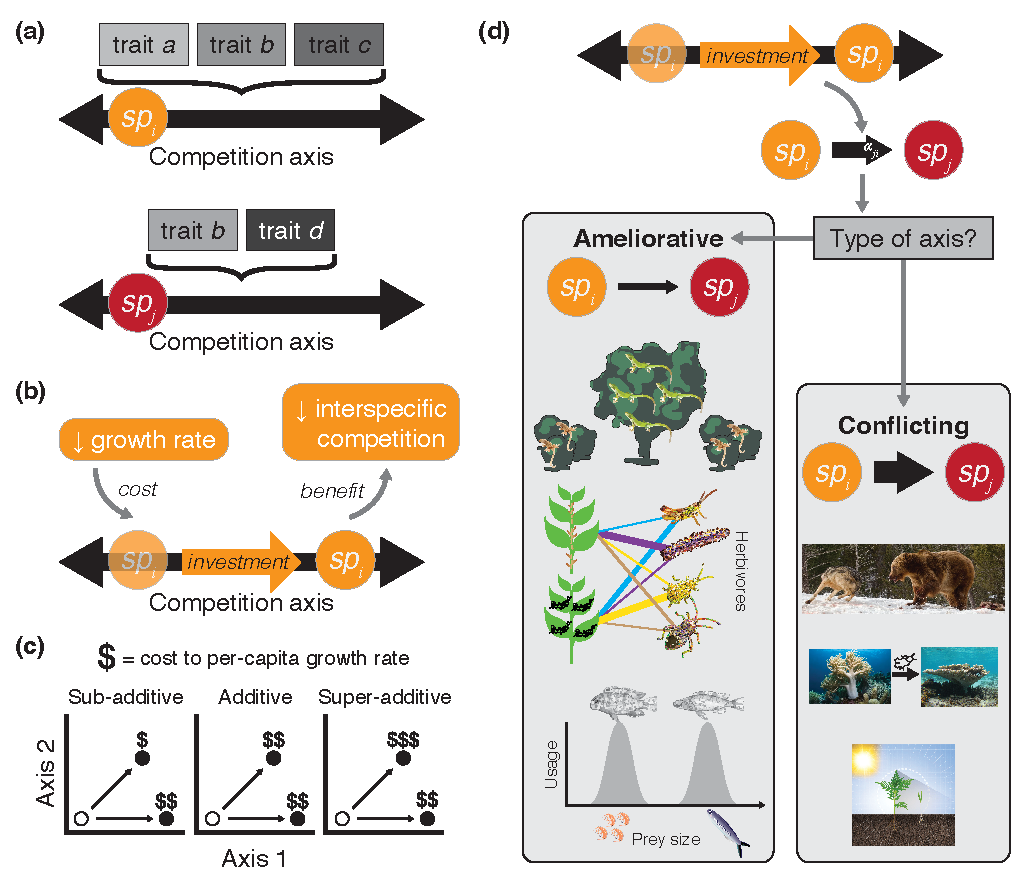
\includegraphics[width=0.9\textwidth,keepaspectratio]{1-diag.pdf}
\caption{Graphical model description.
% 
(a) Competition axes consist of suites of traits that together affect competition
similarly. Traits for a given axis can differ among species.
% 
(b) If species $i$ evolves an increase in a competition axis, this reduces its
per-capita growth rate and the effects of competition species $i$ experiences 
from other species in the community.
% 
(c) The cost associated with investing in multiple axes depends on whether 
tradeoffs are sub-additive, additive, or super-additive. 
Note that arrows within plots in this panel are all the same length.
% 
(d) Investment by species $i$ can either increase or decrease its effect on other
species in the community, depending on the type of competition axis it invests in.
Investment in an ameliorative axis by species $i$ reduces the effect of $i$ on all
other species.
The first example shown is behavioral avoidance of areas where heterospecifics
forage.
Next, investment in defensive traits that cause natural enemies to have 
differing effects on hosts can reduce apparent competition between hosts.
Lastly, multivariate traits can contribute to reduced resource-use overlap
between consumer species.
Investment in a conflicting axis by species $i$ increases the effect of $i$ on all
other species.
Traits that could contribute to conflicting axes include 
aggressive behavior toward heterospecifics near food sources,
chemical suppression of competitors for space, and
rapid growth that shades nearby plants.}
\label{fig:model-description}
\end{figure}




\begin{figure}[ht!]
\centering
\includegraphics{2-outcomes_q2.pdf}
\caption{Unique axis values for surviving species in 2-axis communities
with varying numbers of species (indicated by color), and 
    for tradeoffs being sub-additive ($\eta < 0$), additive ($\eta = 0$), or 
    super-additive ($\eta > 0$).
    The lines in the additive case show the locations of the neutrally stable rings.
    Both axes are neutral (i.e., $\mathbf{d} = \{ 0, 0 \}$) to show only
    the effects of axis investment on the focal species.}
\label{fig:two-axis-outcomes}
\end{figure}






\begin{figure}[ht!]
\centering
\includegraphics[width=0.6\textwidth,keepaspectratio]{3-comm.pdf}
\caption{Effects of axis strength and species investments on 
how permissive communities are to coexistence.
(a) How conflicting and ameliorative axis strength affect scaled community size,
for different communities (indicated by color) and tradeoffs
(solid for super-additive, dashed for sub-additive).
Scaled community size
($\sum_j^n{N_j \text{exp} \{ -\mathbf{v}_{j}^{\text{T}} \mathbf{D} \mathbf{v}_j \}}$)
represents the community abundance accounting
for the effect of species' axes on competition experienced by others in the
community. 
A lower value indicates greater invasibility.
In each sub-panel, the non-focal axis strength is fixed at 0.6.
Crosses indicate points where a community type is no longer stable,
and roman numerals indicate the community represented in panel (b).
(b) Invasibility of some communities representing how tradeoffs and species
investments influence coexistence.
Points in these plots indicate the axis values for equilibrium resident species, and 
numbers inside these points indicate the number of species at each point.
The background color shows what happens when a third species is added:
This invader either is excluded (white), 
excludes one or more residents (orange or pink), or 
coexists with residents to form a new, 3-species community (purple).
Note that ii and v show the same community at different axis strengths.
}
\label{fig:comms-d}
\end{figure}

\begin{figure}[ht!]
\centering
\includegraphics{4-stab.pdf}
\caption{Effects of the number of species investing in the conflicting axis
in 10-species communities with super-additive tradeoffs on 
(a) conflicting-axis investment per species,
(b) ameliorative-axis investment per species, and 
(c) scaled community size (inversely related to invasibility).
Color indicates whether the conflicting axis is strong ($d_{\text{conf}} = 1$),
moderate ($d_{\text{conf}} = 0.5$), or weak ($d_{\text{conf}} = 0.1$).
The ameliorative axis was fixed at $d_{\text{amel}} = 0.5$.
\label{fig:stabilizers}
}
\end{figure}




\begin{figure}[ht!]
\centering
\includegraphics[width=0.9\textwidth,keepaspectratio]{5-stoch.pdf}
\caption{Examples of how stochasticity affects tradeoffs, 
possible communities, and invasibility.
Shown are the effects of axis-evolution stochasticity when
(a) variance is equal among axes and tradeoffs are super-additive and 
(b) variance is unequal among axes and tradeoffs are sub-additive.
The upper row of each sub-panel shows the trajectories in axis space
for 4 species started under each scenario.
Open points indicate starting axis values.
Closed points indicate ending axis values, and 
numbers inside these points indicate the number of species at each point.
Gray shaded curves outside each plot show the probability density for
the normal distributions used to generate stochasticity in the
conflicting (top curve) or ameliorative (right curve) axis.
The lower row shows scaled community size through time for each community
in the top row;
a lower scaled community size indicates greater invasibility.
The first 1,000 time steps are removed to better highlight differences
between communities after the initial period of population expansions.
}
\label{fig:stochasticity}
\end{figure}



\clearpage


\section*{Supplemental Information}

\renewcommand{\thefigure}{S\arabic{figure}}
\renewcommand{\theequation}{S\arabic{equation}}
\renewcommand{\thetable}{S\arabic{table}}
\setcounter{equation}{0}
\setcounter{figure}{0}
\setcounter{table}{0}


% Note: this should go into a separate document eventually

\section*{Matrix derivatives in quantitative genetics equations}

As in the main text, $^{\textrm{T}}$ indicates transposition,
multiplication between matrices is always matrix multiplication, and
bold face indicates a matrix.
Also note that both $\mathbf{C}$ and $\mathbf{D}$ are symmetrical,
so $\mathbf{C} + \mathbf{C}^{\textrm{T}} = 2 \; \mathbf{C}$ and
$\mathbf{D} + \mathbf{D}^{\textrm{T}} = 2 \; \mathbf{D}$.


We can combine the equations in the Methods section as such:

\begin{equation} \label{eq:fitness-full}
\begin{split}
    F_{i,t+1} &= \exp \left\{
        r_0 - f \; \mathbf{v}_{i,t}^{\textrm{T}} \; \mathbf{C} \; \mathbf{v}_{i,t} -
        \alpha_0 \;\textrm{e}^{- \mathbf{v}_{i,t}^{\textrm{T}} \mathbf{v}_{i,t} } \mathbf{\Omega}_{i,t}
        \right\} \\
        \mathbf{\Omega}_{i,t} &\equiv N_{i,t} +
            \sum_{j \ne i}^{n}{ N_{j,t} \textrm{e}^{
            - \mathbf{v}_{j,t}^{\textrm{T}}
            \mathbf{D} \mathbf{v}_{j,t} } }
        \textrm{.}
\end{split}
\end{equation}

\noindent where $\mathbf{\Omega}_i$ represents the community abundance scaled
for the effect other species' axes values has on competition
experienced by species $i$.
Hereafter we will refer to $\mathbf{\Omega}_i$ as the scaled community size.




\subsection*{Axis evolution}

From the main text and above, we know that

\begin{equation}\label{eq:main-text-info-axis-change}
\begin{split}
    F_{i,t+1} &= \exp \left\{
        r_0 - f \; \mathbf{v}_{i,t}^{\textrm{T}} \; \mathbf{C} \; \mathbf{v}_{i,t} -
        \alpha_0 \;\textrm{e}^{- \mathbf{v}_{i,t}^{\textrm{T}} \mathbf{v}_{i,t} } \mathbf{\Omega}_{i,t}
        \right\} \\
    \mathbf{v}_{i,t+1} &= \mathbf{v}_{i,t} + \left( \frac{1}{F_{i,t+1}}
        \frac{\partial F_{i,t+1}}{\partial \mathbf{v}_{i,t}} \right) \sigma^2_i
    \textrm{.}
\end{split}
\end{equation}


The partial derivative of fitness in relation to axes for species $i$ is


\begin{equation*}
\begin{split}
    \frac{\partial F_{i,t+1}}{\partial \mathbf{v}_{i,t}} &=
        \exp \left\{
            r_0
            - f \mathbf{v}_{i,t}^{\textrm{T}} \mathbf{C} \mathbf{v}_{i,t}
            - \alpha_0  \mathbf{\Omega}_{i,t} \,
                \textrm{e}^{- \mathbf{v}_{i,t}^{\textrm{T}} \mathbf{v}_{i,t}}
        \right\}
        \frac{\partial \!
            \left(
                r_0
                - f \; \mathbf{v}_{i,t}^{\textrm{T}} \; \mathbf{C} \; \mathbf{v}_{i,t}
                - \alpha_0 \; \mathbf{\Omega}_{i,t} \;
                    \textrm{e}^{- \mathbf{v}_{i,t}^{\textrm{T}} \mathbf{v}_{i,t}}
            \right)
            }{ \partial \mathbf{v}_{i,t} } \\
     &=
        \exp \left\{
            r_0
            - f \mathbf{v}_{i,t}^{\textrm{T}} \mathbf{C} \mathbf{v}_{i,t}
            - \alpha_0  \mathbf{\Omega}_{i,t} \,
                \textrm{e}^{- \mathbf{v}_{i,t}^{\textrm{T}} \mathbf{v}_{i,t}}
        \right\}
        \left[
            - 2 f \mathbf{v}_{i,t}^{\textrm{T}} \mathbf{C}
            - \alpha_0 \, \mathbf{\Omega}_{i,t} \,
                \textrm{e}^{- \mathbf{v}_{i,t}^{\textrm{T}} \mathbf{v}_{i,t} } \:
                \frac{\partial \! \left( - \mathbf{v}_{i,t}^{\textrm{T}} \mathbf{v}_{i,t} \right)
                    }{ \partial \mathbf{v}_{i,t} }
        \right] \\[2ex]
    \frac{ \partial F_{i,t} }{ \partial \mathbf{v}_{i,t} } &=
        \exp \left\{
            r_0
            - f \mathbf{v}_{i,t}^{\textrm{T}} \mathbf{C} \mathbf{v}_{i,t}
            - \alpha_0  \mathbf{\Omega}_{i,t} \,
                \textrm{e}^{- \mathbf{v}_{i,t}^{\textrm{T}} \mathbf{v}_{i,t}}
        \right\}
        \left[
            2 \alpha_0 \mathbf{\Omega}_{i,t} \,
                \textrm{e}^{- \mathbf{v}_{i,t}^{\textrm{T}} \mathbf{v}_{i,t}} \:
                \mathbf{v}_{i,t}^{\textrm{T}}
            - 2 f \mathbf{v}_{i,t}^{\textrm{T}} \mathbf{C}
        \right]
    \textrm{.}
\end{split}
\end{equation*}



Combining above with equation \ref{eq:main-text-info-axis-change}, we find that axis values at
time $t+1$ are

\begin{equation} \label{eq:supp-axis-change-full}
    \mathbf{v}_{i,t+1} = \mathbf{v}_{i,t} + 2 \sigma_i^2
    \left(
        \alpha_0 \, \mathbf{\Omega}_{i,t} \:
            \textrm{e}^{- \mathbf{v}_{i,t}^{\textrm{T}} \mathbf{v}_{i,t}} \:
            \mathbf{v}_{i,t}^{\textrm{T}}
        - f \, \mathbf{v}_{i,t}^{\textrm{T}} \: \mathbf{C}
    \right)
    \textrm{.}
\end{equation}


\subsection*{Jacobian matrix}

The $n(q+1) \times n(q+1)$ Jacobian matrix consists of 

\begin{itemize}
\item $n^2$ blocks of size $q \times q$ containing
    $\partial \mathbf{v}_{i,t+1} / \partial \mathbf{v}_{\zeta,t}$
\item $n^2$ blocks of size $1 \times q$ containing
    $\partial \mathbf{v}_{i,t+1} / \partial N_{\zeta,t}$
\item $n^2$ blocks of size $q \times 1$ containing
    $\partial N_{i,t+1} / \partial \mathbf{v}_{\zeta,t}$
\item $n^2$ blocks of size $1 \times 1$ containing
    $\partial N_{i,t+1} / \partial N_{\zeta,t}$
\end{itemize}


for all $i \in \{ 1, \: \ldots \, , \: n \}$
and $\zeta \in \{ 1, \: \ldots \, , \: n \}$.


The partial derivatives of species $i$ axes at time $t+1$ with respect
to species $i$ axes at time $t$ are

\begin{equation*}
\begin{split}
    \frac{ \partial \, \mathbf{v}_{i,t+1} }{ \partial \, \mathbf{v}_{i,t} } &=
        \frac{ \partial \, \mathbf{v}_{i,t} }{ \partial \, \mathbf{v}_{i,t} } +
        2 \; \sigma_i^2
        \left(
            \frac{ \partial \;
                \alpha_0 \; \mathbf{\Omega}_{i,t} \;
                    \textrm{e}^{-\mathbf{v}_{i,t}^{\textrm{T}} \mathbf{v}_{i,t}} \,
                    \mathbf{v}_{i,t}^{\textrm{T}}}{\partial \; \mathbf{v}_{i,t} } -
            \frac{ \partial \; f \, \mathbf{v}_{i,t}^{\textrm{T}} \mathbf{C}}{\partial \; \mathbf{v}_{i,t} }
        \right) \\
    &=
        \mathbf{I} +
        2 \; \sigma_i^2
        \left[
            \alpha_0 \; \mathbf{\Omega}_{i,t} \,
            \left(
                \textrm{e}^{-\mathbf{v}_{i,t}^{\textrm{T}} \mathbf{v}_{i,t}} +
                \frac{ \partial \;
                        \textrm{e}^{-\mathbf{v}_{i,t}^{\textrm{T}} \mathbf{v}_{i,t}}
                        }{\partial \; \mathbf{v}_{i,t} } \, \mathbf{v}_{i,t}^{\textrm{T}}
            \right) -
            f \, \mathbf{C}^{\textrm{T}}
            \right] \\[2ex]
    \frac{ \partial \, \mathbf{v}_{i,t+1} }{ \partial \, \mathbf{v}_{i,t} } &= \mathbf{I} + 2 ~ \sigma_i^2 ~
        \left[
            \alpha_0 ~ \mathbf{\Omega}_{i,t} ~ \textrm{e}^{ - \mathbf{v}_{i,t}^{\textrm{T}} \mathbf{v}_{i,t} }
            \left(
                \mathbf{I} - 2 ~ \mathbf{v}_{i,t} \mathbf{v}_{i,t}^{\textrm{T}}
            \right) -
            f \: \mathbf{C}^{\textrm{T}}
        \right]
    \textrm{,}
\end{split}
\end{equation*}

\noindent where $\mathbf{I}$ is a $q \times q$ identity matrix.


Next we have the partial derivatives of species $i$ axes at time $t+1$ with respect to 
species $k$ axes at time $t$, where $k \ne i$.
To calculate this, it's useful to rearrange equation \ref{eq:axes-change-full} and
extract the portion that includes $\mathbf{v}_{k,t}$:


\begin{equation*}
\begin{split}
    \mathbf{v}_{i,t+1} &= \mathbf{v}_{i,t} + 2 \; \sigma_i^2
    \left[
        \left(
            N_{k,t} \; \textrm{e}^{ -\mathbf{v}_{k,t}^{\textrm{T}} \mathbf{D}
            \mathbf{v}_{k,t} } + \mathbf{\Phi}_{i,t}
        \right)
        \left(
            \alpha_0 \; \textrm{e}^{-\mathbf{v}_{i,t}^{\textrm{T}}
            \mathbf{v}_{i,t} } \; \mathbf{v}_{i,t}^{\textrm{T}}
        \right)
        - f \: \mathbf{v}_{i,t}^{\textrm{T}} \mathbf{C}
    \right] \\
    \mathbf{\Phi}_{i,t} &= N_{i,t} + \sum_{j \ne i, j \ne k}^{n}{
        N_{j,t} \; \textrm{e}^{- \mathbf{v}_{j,t}^{\textrm{T}}
        \mathbf{D} \mathbf{v}_{j,t} } }
    \textrm{.}
\end{split}
\end{equation*}

From this we calculated the partial derivative of $\mathbf{v}_{i,t+1}$ in relation to
$\mathbf{v}_{k,t}$


\begin{equation*}
\begin{split}
    \frac{ \partial \: \mathbf{v}_{i,t+1} }{ \partial \: \mathbf{v}_{k,t} } &=
        \frac{ \partial \: \mathbf{v}_{i,t} }{ \partial \: \mathbf{v}_{k,t} } +
        2 \; \sigma_i^2 \;
        \left[
            \frac{ \partial \:
                \left(
                    N_{k,t} \textrm{e}^{- \mathbf{v}_{k,t}^{\textrm{T}} \mathbf{D}
                    \mathbf{v}_{k,t}} + \mathbf{\Phi}_{i,t}
                \right)
                \left(
                    \alpha_0 \; \textrm{e}^{ - \mathbf{v}_{i,t}^{\textrm{T}}
                    \mathbf{v}_{i,t} } \mathbf{v}_{i,t}^{\textrm{T}}
                \right)
            }{ \partial \:  \mathbf{v}_{k,t} } -
            \frac{ \partial \:  f \, \mathbf{v}_{i,t}^{\textrm{T}} \mathbf{C} }{
            \partial \: \mathbf{v}_{k,t} }
        \right] \\
    &= 2 \; \sigma_i^2 \; \alpha_0 \; N_{k,t} \; \mathbf{v}_{i,t} \;
        \textrm{e}^{ - \mathbf{v}_{i,t}^{\textrm{T}}
        \mathbf{v}_{i,t} } \; 
        \frac{ \partial \:
                \textrm{e}^{
                    - \mathbf{v}_{k,t}^{\textrm{T}} \mathbf{D} \mathbf{v}_{k,t}
                    }
            }{ \partial \:  \mathbf{v}_{k,t} } \\
    &= 2 \; \sigma_i^2 \; \alpha_0 \; N_{k,t} \; \mathbf{v}_{i,t} \;
        \textrm{e}^{
                    - \mathbf{v}_{k,t}^{\textrm{T}} \mathbf{D} \mathbf{v}_{k,t}
                    - \mathbf{v}_{i,t}^{\textrm{T}} \mathbf{v}_{i,t}
                } \;
        \left[ 
            - 2 \, \mathbf{v}_{k,t}^{\textrm{T}} \, \mathbf{D}
        \right] \\
    \frac{ \partial \: \mathbf{v}_{i,t+1} }{ \partial \: \mathbf{v}_{k,t}} &=
        -4 \; \sigma_i^2 \; \alpha_0 \; N_{k,t} \; \mathbf{v}_{i,t} \;
        \textrm{e}^{
                    - \mathbf{v}_{k,t}^{\textrm{T}} \mathbf{D} \mathbf{v}_{k,t}
                    - \mathbf{v}_{i,t}^{\textrm{T}} \mathbf{v}_{i,t}
                } \;
        \mathbf{v}_{k,t}^{\textrm{T}} \; \mathbf{D}
    \textrm{.} \\
\end{split}
\end{equation*}

The partial derivatives of species $i$ axes in relation to species $i$ 
and species $k$ abundances are

\begin{equation*}
\begin{split}
    \frac{ \partial \: \mathbf{v}_{i,t+1} }{ \partial \: N_{i,t} } &=
        2 \; \sigma_i^2 \; \alpha_0 \; \mathbf{v}_{i,t} \;
        \textrm{e}^{ - \mathbf{v}_{i,t}^{\textrm{T}} \mathbf{v}_{i,t} } \\
    \frac{ \partial \: \mathbf{v}_{i,t+1} }{ \partial \: N_{k,t} } &=
        2 \; \sigma_i^2 \; \alpha_0 \; \mathbf{v}_{i,t} \;
        \textrm{e}^{ - \mathbf{v}_{k,t}^{\textrm{T}} \mathbf{D} \mathbf{v}_{k,t}
            - \mathbf{v}_{i,t}^{\textrm{T}} \mathbf{v}_{i,t} }
    \textrm{.} \\
\end{split}
\end{equation*}




For partial derivatives of abundances in relation to the other state variables,
we use the following equations from above:


\begin{equation*}
\begin{split}
    N_{i,t+1} &= N_{i,t} \; F_{i,t+1} \\
    F_{i,t+1} &=  \exp \left\{
        r_0 - f \, \mathbf{v}_{i,t}^{\text{T}} \, \mathbf{C} \, \mathbf{v}_{i,t} - 
        \alpha_0 \, \text{e}^{-\mathbf{v}_{i,t}^{\text{T}} \, \mathbf{v}_{i,t}} \,
        \Omega_{i,t}
    \right\} \\
    \Omega_{i,t} &= N_{i,t} + \sum_{j \ne i}^{n}{ N_j \:
        \text{e}^{- \mathbf{v}_{j,t}^{\text{T}} \, \mathbf{D} \, \mathbf{v}_{j,t} } }
    \textrm{.} \\
\end{split}
\end{equation*}



Using these, we have the following derivatives of abundances in relation
to axes:

\begin{equation*}
\begin{split}
    \frac{ \partial N_{i,t+1} }{ \partial \mathbf{v}_{i,t} } &= 
        2 \, F_{i,t+1} \,  N_{i,t}
        \left(
            \alpha_0 \, \Omega_{i,t} \, \text{e}^{ -\mathbf{v}_{i,t}^{\text{T}}
            \mathbf{v}_{i,t} } \, \mathbf{v}_{i,t}^{\text{T}}
            - f \, \mathbf{v}_{i,t}^{\text{T}} \, \mathbf{C}
        \right) \\
    \frac{ \partial N_{i,t+1} }{ \partial \mathbf{v}_{k,t} } &= 
        2 \, F_{i,t+1} \, N_{i,t} \, N_{k,t} \, \alpha_0 \: 
        \text{e}^{ -\mathbf{v}_{i,t}^{\text{T}} \mathbf{v}_{i,t} -
            \mathbf{v}_{k,t}^{\text{T}} \mathbf{D} \mathbf{v}_{k,t} } \:
        \mathbf{v}_{k,t}^{\text{T}} \, \mathbf{D}
    \textrm{.}
\end{split}
\end{equation*}

We also have the following derivatives of abundances at time $t+1$ in relation
to those at time $t$:

\begin{equation*}
\begin{split}
    \frac{ \partial N_{i,t+1} }{ \partial N_{i,t} } &= 
        F_{i,t+1}
        \left(
            1 - N_{i,t} \: \alpha_0 \: 
            \text{e}^{ -\mathbf{v}_{i,t}^{\text{T}} \mathbf{v}_{i,t} } 
        \right) \\
    %
    \frac{ \partial N_{i,t+1} }{ \partial N_{k,t} } &= 
        - F_{i,t+1} \: N_{i,t} \: \alpha_0 \: 
        \text{e}^{ -\mathbf{v}_{i,t}^{\text{T}} \mathbf{v}_{i,t} -
            \mathbf{v}_{k,t}^{\text{T}} \mathbf{D} \mathbf{v}_{k,t} } 
    \textrm{.}
\end{split}
\end{equation*}











% ========================================================================================
% ========================================================================================
% ========================================================================================
% ========================================================================================
% ========================================================================================
% ========================================================================================
% ========================================================================================






\section*{Two-axis equilibrium solutions}

For these solutions, we will no longer use matrix notation.
Also, since all axes have the same costs, benefits, and
non-additive effects, solutions for axis 1 and 2 are the same.
Only solutions for axis 1 are presented.
We use a hat to distinguish equilibrium values
($\hat{Z}$ for parameter $Z$).
Lastly, because $\mathbf{C}$ is symmetrical, only has 2 rows and columns, and
differs only on the off-diagonals, there is only one $\eta$ value.


\subsection*{Axis values}

The two axes for species $i$ change as follows:

\begin{equation*}
\begin{split}
    v_{i1,t+1} &= v_{i1,t} + 2 \; \sigma^2
    \left[
        \alpha_0 \; \Omega_{i,t} \;
            \textrm{e}^{-v_{i1,t}^2 - v_{i2,t}^2} \; v_{i1,t}
        - f \; ( v_{i1,t} + \eta \; v_{i2,t} )
    \right] \\
    v_{i2,t+1} &= v_{i2,t} + 2 \; \sigma^2
    \left[
        \alpha_0 \; \Omega_{i,t} \;
            \textrm{e}^{-v_{i2,t}^2 - v_{i1,t}^2} \; v_{i2,t}
        - f \; ( v_{i2,t} + \eta \; v_{i1,t} )
    \right] \\
    \Omega_{i,t} &\equiv N_{i,t} +
        \sum_{j \ne i}^{n}{ N_{j,t} \; \textrm{e}^{
                - d_1 v_{j1,t}^2 - d_2 v_{j2,t}^2 } }
    \textrm{.}
\end{split}
\end{equation*}


We'll now drop indices for species and time because we are
focusing on just one species and time point.



At equilibrium (assuming that $\sigma > 0$),

\begin{equation}
\begin{split}
    0 &= \alpha_0 \; \hat{\Omega} \;
            \textrm{e}^{-\hat{v}_{1}^2 - \hat{v}_{2}^2} \; \hat{v}_{1}
        - f \; ( \hat{v}_{1} + \eta \; \hat{v}_{2} ) \\
    0 &=
        \alpha_0 \; \hat{\Omega} \;
            \textrm{e}^{-\hat{v}_{2}^2 - \hat{v}_{1}^2} \; \hat{v}_{2}
        - f \; ( \hat{v}_{2} + \eta \; \hat{v}_{1} )
    \textrm{.}
\end{split}
\label{eq:two-axes-v-eq1}
\end{equation}


\noindent Thus, we have

\begin{equation*}
\begin{split}
    \alpha_0 \; \hat{\Omega} \; \textrm{e}^{-\hat{v}_{1}^2 - \hat{v}_{2}^2} &=
        \frac{ f \; ( \hat{v}_{1} + \eta \; \hat{v}_{2} ) }{ \hat{v}_{1} } \\
    \alpha_0 \; \hat{\Omega} \; \textrm{e}^{-\hat{v}_{1}^2 - \hat{v}_{2}^2} &=
        \frac{ f \; ( \hat{v}_{2} + \eta \; \hat{v}_{1} ) }{ \hat{v}_{2} }
    \textrm{.}
\end{split}
\end{equation*}


\noindent Combining these leads to

\begin{equation*}
\begin{split}
    f \; ( \hat{v}_{1} + \eta \; \hat{v}_{2} ) \; \hat{v}_{2} &=
        f \; ( \hat{v}_{2} + \eta \; \hat{v}_{1} ) \; \hat{v}_{1} \\
    f \hat{v}_{1} \hat{v}_{2} + \eta \hat{v}_{2}^2 &=
        f \hat{v}_{1} \hat{v}_{2} + \eta \hat{v}_{1}^2 \\
    \eta \hat{v}_{2}^2 &= \eta \hat{v}_{1}^2 \\
    \hat{v}_{1} &= \hat{v}_{2}
    \textrm{.}
\end{split}
\end{equation*}

Since all $v$ must be $\ge 0$ (hence no $\pm$ in the equation above),
either $\hat{v}_{1} = \hat{v}_{2}$ or not (when $\eta = 0$).
Plugging in $\hat{v}_{1} = \hat{v}_{2}$ into equation \ref{eq:two-axes-v-eq1}
gives us

\begin{equation*}
\begin{split}
    0 &= \alpha_0 \; \hat{\Omega} \; \textrm{e}^{-2 \; \hat{v}_{1}^2 } \; \hat{v}_{1}
        - f \; ( \hat{v}_{1} + \eta \; \hat{v}_{1} ) \\
    &= \hat{v}_{1} \left[ \alpha_0 \; \hat{\Omega} \; \textrm{e}^{-2 \; \hat{v}_{1}^2 }
        - f \; ( 1 + \eta ) \right]
    \textrm{.}
\end{split}
\end{equation*}

\noindent One solution is $\hat{v}_{1} = 0$, but if $\hat{v}_{1} \ne 0$


\begin{equation}
\begin{split}
    \alpha_0 \; \hat{\Omega} \; \textrm{e}^{-2 \; \hat{v}_{1}^2 } &=
        f \; ( 1 + \eta ) \\
    -2 \; \hat{v}_{1}^2 &=
        \log \left( \frac{ f \; ( 1 + \eta ) }{ \alpha_0 \; \hat{\Omega} } \right) \\
    \hat{v}_{1} &= \sqrt{\frac{1}{2}
        \log \left( \frac{ \alpha_0 \; \hat{\Omega} }{ f \; ( 1 + \eta ) } \right) }
    \textrm{.}
\end{split}
\label{eq:two-axes-v-eq5}
\end{equation}



When $\eta = 0$ and at least one of the two axes $\ne 0$,
axes are constrained by their distance
from the origin: $\sqrt{\hat{v}_{1}^2 + \hat{v}_{2}^2}$.
When $\hat{v}_{1} \ne 0$, this distance is

\begin{equation*}
\begin{split}
    0 &= \alpha_0 \; \hat{\Omega} \;
            \textrm{e}^{-\hat{v}_{1}^2 - \hat{v}_{2}^2} \; \hat{v}_{1}
        - f \; \hat{v}_{1} \\
    0 &= \alpha_0 \; \hat{\Omega} \;
        \textrm{e}^{- ( \hat{v}_{1}^2 + \hat{v}_{2}^2) }
        - f \\
    \log \left( \frac{\alpha_0 \; \hat{\Omega}}{ f } \right) &=
        \hat{v}_{1}^2 + \hat{v}_{2}^2 \\
     \sqrt{ \hat{v}_{1}^2 + \hat{v}_{2}^2 } &=
        \sqrt{ \log \left( \frac{\alpha_0 \; \hat{\Omega}}{ f } \right)}
    \textrm{.}
\end{split}
\end{equation*}

\noindent So the relationship between axes when $\eta = 0$ is

$$
    \hat{v}_{1} =
    \sqrt{
        \log \left( \frac{\alpha_0 \; \hat{\Omega}}{ f } \right) -
        \hat{v}_{2}^2
    }
    \textrm{,}
$$

\noindent when $\hat{v}_{2}^2 \ge \log (\alpha_0 \hat{\Omega} / f)$.

We've shown solutions for when $v_1 = v_2$ and when $\eta = 0$, but
when one axis is zero but the other is not (and $\eta$ isn't necessarily 0),
we get the following (for $v_1 \ne 0$ and $v_2 = 0$):

\begin{equation}
\begin{split}
    0 &=
        \alpha_0 \; \hat{\Omega} \;
            \textrm{e}^{-\hat{v}_{1}^2 - \hat{v}_{2}^2} \; \hat{v}_{1}
        - f \; ( \hat{v}_{1} + \eta \; \hat{v}_{2} ) \\
    0 &=
        \alpha_0 \; \hat{\Omega} \;
            \textrm{e}^{-\hat{v}_{1}^2} \; \hat{v}_{1}
        - f \; \hat{v}_{1} \\
    0 &=
        \alpha_0 \; \hat{\Omega} \;
            \textrm{e}^{-\hat{v}_{1}^2} - f \\
    \frac{f}{\alpha_0 \; \hat{\Omega}} &=
         \frac{1}{\textrm{e}^{\hat{v}_{1}^2}} \\
    \hat{v}_{1} &= \sqrt{ \log \left( \frac{\alpha_0 \; \hat{\Omega}}{f} \right) }
\end{split}
\label{eq:two-axes-v1-nonzero-v2-zero}
\end{equation}







% -----------------------------------------------------------------
% -----------------------------------------------------------------







\subsection*{Scaled community size}

Fitness for the species is written as

$$
    F = \exp \left\{
        r_0 - f ( {v}_{1}^2 + 2 \eta {v}_{1} {v}_{2} + {v}_{2}^2 ) -
        \alpha_0 \, \textrm{e}^{ - {v}_{1}^2 - {v}_{2}^2 } \, \Omega
    \right\}
    \textrm{.}
$$


\noindent At equilibrium,

\begin{equation}
    0 = r_0 - f ( \hat{v}_{1}^2 + 2 \eta \hat{v}_{1} \hat{v}_{2} + \hat{v}_{2}^2 ) -
        \alpha_0 \, \textrm{e}^{ - {v}_{1}^2 - {v}_{2}^2 } \, \Omega
    \textrm{.}
\label{eq:two-axes-omega-equil-start}
\end{equation}


\noindent When $\hat{v}_1 = \hat{v}_2$, we can insert our answer from
\ref{eq:two-axes-v-eq5} to get

\begin{equation*}
\begin{split}
    0 &= r_0 - 2 \; f \; \hat{v}_{1}^2 ( 1 + \eta ) -
        \alpha_0 \textrm{e}^{ -2 \; \hat{v}_{1}^2 } \hat{\Omega} \\
    r_0 &= 2 f ( 1 + \eta ) \left[
        \frac{1}{2}
        \log \left( \frac{ \alpha_0 \; \hat{\Omega} }{ f \; ( 1 + \eta ) } \right)
    \right] +
        \alpha_0 \textrm{e}^{ -2 \;
            \left[
                \frac{1}{2} \log \left(
                    \frac{ \alpha_0 \; \hat{\Omega} }{ f \; ( 1 + \eta ) }
                \right)
            \right]
        } \hat{\Omega} \\
    r_0 &= f ( 1 + \eta ) \log \left(
        \frac{ \alpha_0 \; \hat{\Omega} }{ f \; ( 1 + \eta ) }
    \right) + f ( 1 + \eta ) \\
    \frac{  r_0 - f ( 1 + \eta ) }{ f ( 1 + \eta ) } &=
        \log \left(
        \frac{ \alpha_0 \; \hat{\Omega} }{ f \; ( 1 + \eta ) }
        \right) \\
    \hat{\Omega} &= \frac{ f \; ( 1 + \eta ) }{ \alpha_0 } \;
        \textrm{e}^{\frac{  r_0 }{ f ( 1 + \eta ) } - 1 }
    \textrm{.}
\end{split}
\end{equation*}

Thus, when $\hat{v}_1 = \hat{v}_2$,
$$
\hat{\Omega} = \frac{ f \; ( 1 + \eta ) }{ \alpha_0 } \;
        \textrm{e}^{\frac{ r_0 }{ f ( 1 + \eta ) } - 1 }
    \textrm{.}
$$


\noindent When $\eta = 0$,

$$
    \hat{\Omega} = \frac{ f }{ \alpha_0 } \; \textrm{e}^{\frac{ r_0 }{ f } - 1 }
    \textrm{.}
$$



If instead $v_1 = 0$ and $v_2 \ne 0$, we can start by simplifying equation
\ref{eq:two-axes-omega-equil-start}

\begin{equation*}
\begin{split}
    0 &= r_0 - f \hat{v}_{1}^2 -
        \alpha_0 \textrm{e}^{ - \hat{v}_{1}^2 } \hat{\Omega} \\
    \hat{\Omega} &= \frac{ r_0 - f \hat{v}_{1}^2 }{ \alpha_0 } \textrm{e}^{ \hat{v}_{1}^2 }
    \textrm{.}
\end{split}
\end{equation*}

Now we combine this with \ref{eq:two-axes-v1-nonzero-v2-zero}

\begin{equation*}
\begin{split}
    \hat{\Omega} &= \frac{ r_0 - f \log \left( \frac{\alpha_0 \hat{\Omega}}{f} \right) }{
        \alpha_0 } \left( \frac{\alpha_0 \; \hat{\Omega}}{f} \right) \\
    1 &= \frac{ r_0 }{ f } - \log \left( \frac{\alpha_0 \hat{\Omega}}{f} \right) \\
    \hat{\Omega} &= \frac{f}{\alpha_0} \textrm{e}^{\frac{r_0}{f} - 1}
    \textrm{.}
\end{split}
\end{equation*}











% -----------------------------------------------------------------
% -----------------------------------------------------------------








\subsection*{Combined solutions}

When $\hat{v}_1 = \hat{v}_2$,

\begin{equation}  \label{eq:two-axes-finals-eta-negative}
\begin{split}
    \hat{\Omega} &= \frac{ f \; ( 1 + \eta ) }{ \alpha_0 } \;
        \textrm{e}^{\frac{  r_0 }{ f ( 1 + \eta ) } - 1 }
        \\
    \hat{v}_1 &= \sqrt{
        \frac{1}{2} \left( \frac{ r_0 }{ f (1 + \eta) } - 1 \right)
    }
    \textrm{.}
\end{split}
\end{equation}


\noindent When $\eta = 0$,

\begin{equation}  \label{eq:two-axes-finals-eta-zero}
\begin{split}
    \hat{\Omega} &= \frac{ f }{ \alpha_0 } \; \textrm{e}^{\frac{ r_0 }{ f } - 1 } \\
    \sqrt{\hat{v}_1^2 + \hat{v}_2^2} &= \sqrt{ \frac{ r_0 }{ f } - 1 } \\
    \hat{v}_1 &= \sqrt{ \frac{ r_0  }{ f } - \hat{v}_2^2 - 1 }
    \textrm{.}
\end{split}
\end{equation}


\noindent When $v_1 \ne 0$, $v_2 = 0$, and $\eta \ne 0$,

\begin{equation}  \label{eq:two-axes-finals-eta-positive}
\begin{split}
    \hat{\Omega} &= \frac{f}{\alpha_0} \textrm{e}^{\frac{r_0}{f} - 1} \\
    \hat{v}_1 &= \sqrt{ \frac{ r_0 }{ f } - 1 }
    \textrm{.}
\end{split}
\end{equation}

\noindent Thus, when $v_1 \ne 0$, $v_2 = 0$, and $\eta \ne 0$, the equilibrium
dynamics match that for when $\eta = 0$, which is not surprising given that
you cannot have a non-additive tradeoff when one axis has a zero value.









% -----------------------------------------------------------------
% -----------------------------------------------------------------








\subsection*{Differences in abundance among species}



This section analyzes a two-species community where each species has one of two potential
outcomes in terms of axis equilibria:
(1) $\hat{v}_1 = \hat{v}_2$ and
(2) $\hat{v}_1 \ne 0 \; \& \; \hat{v}_2 = 0$.
I'm not discussing when $\eta = 0$ because that's not biologically very realistic
and those results are likely an artifact of the model structure.


\subsubsection*{At the same axis equilibrium:}

The first scenario is when both species have $\hat{v}_1 = \hat{v}_2$.
If this is the case, then from above, we know that

\begin{equation*}
\begin{split}
    \hat{v}_{11} &= \hat{v}_{12} = \hat{v}_{21} = \hat{v}_{22} = \sqrt{\frac{1}{2}
        \left( \frac{r_0}{f (1 + \eta)} - 1 \right)} \\
    \hat\Omega_1 &= \hat\Omega_2 = \frac{f (1 + \eta)}{\alpha_0}
        \text{e}^{\frac{r_0}{f (1 + \eta)} - 1}
    \text{.}
\end{split}
\end{equation*}

Because all axes and scale community sizes are equal, and because of our
definition of $\Omega$ from equation ??
% \ref{eq:fitness-full}

\begin{equation} \label{eq:two-axes-v1-v2-equal-N1-N2}
\begin{split}
    \hat{N}_1 + \hat{N}_2 \: \text{e}^{-\hat{v}_{11}^2 (d_1 + d_2)} &=
        \hat{N}_2 + \hat{N}_1 \: \text{e}^{-\hat{v}_{11}^2 (d_1 + d_2)} \\
    \hat{N}_1 \left( 1 - \text{e}^{-\hat{v}_{11}^2 (d_1 + d_2)} \right) &=
        \hat{N}_2 \left( 1 - \text{e}^{-\hat{v}_{11}^2 (d_1 + d_2)} \right) \\
    \hat{N}_1 &= \hat{N}_2
    \text{.}
\end{split}
\end{equation}

\noindent Combining the above two sets of equations to solve for $\hat{N}_1$ in
terms of parameters:


\begin{equation} \label{eq:two-axes-v1-v2-equal-N}
\begin{split}
    \hat\Omega_1 &= \hat{N}_1 + \hat{N}_2 \: \text{e}^{-d_1 \hat{v}_{21}^2 -
        d_2 v_{22}^2} \\
    \frac{f (1 + \eta)}{\alpha_0} \text{e}^{\frac{r_0}{f (1 + \eta)} - 1} &=
        \hat{N}_1 + \hat{N}_1 \: \text{e}^{- \hat{v}_{11}^2 (d_1 + d_2)} \\
    \frac{f (1 + \eta)}{\alpha_0} \text{e}^{\frac{r_0}{f (1 + \eta)} - 1} &=
        \hat{N}_1 \left[ 1 + \text{e}^{- \frac{1}{2} \left(
            \frac{r_0}{f (1 + \eta)} - 1 \right) (d_1 + d_2)} \right] \\
    \hat{N}_1 &= \frac{f (1 + \eta)}{\alpha_0  \left[ 1 + \text{e}^{- \frac{1}{2} \left(
        \frac{r_0}{f (1 + \eta)} - 1 \right) (d_1 + d_2)} \right] } \;
        \text{e}^{\frac{r_0}{f (1 + \eta)} - 1}
    \text{.}
\end{split}
\end{equation}


This extends to $n$ species as follows:

\begin{equation} \label{eq:two-axes-v1-v2-equal-N-n-species}
    \hat{N}_1 = \frac{f (1 + \eta)}{\alpha_0  \left[ 1 + \text{e}^{- \frac{1}{2} \left(
        \frac{r_0}{f (1 + \eta)} - 1 \right) (d_1 + d_2)}  (n - 1) \right] } \;
        \text{e}^{\frac{r_0}{f (1 + \eta)} - 1}
    \text{.}
\end{equation}




Similarly, when both species have $\hat{v}_1 \ne 0 \; \& \; \hat{v}_2 = 0$:

\begin{equation*}
\begin{split}
    \hat{v}_{11} &= \hat{v}_{21} = \sqrt{ \frac{ r_0 }{ f } - 1 } \\
    \hat{v}_{12} &= \hat{v}_{22} = 0 \\
    \hat\Omega_1 &= \hat\Omega_2 = \frac{f}{\alpha_0} \textrm{e}^{\frac{r_0}{f} - 1}
    \text{.}
\end{split}
\end{equation*}

\noindent Therefore,

\begin{equation} \label{eq:two-axes-v1-nonzero-v2-zero-N1-N2}
\begin{split}
    \hat{N}_1 + \hat{N}_2 \: \text{e}^{- d_1 \hat{v}_{11}^2 } &=
        \hat{N}_2 + \hat{N}_1 \: \text{e}^{- d_1 \hat{v}_{11}^2 } \\
    \hat{N}_1 \left( 1 - \text{e}^{- d_1 \hat{v}_{11}^2 } \right) &=
        \hat{N}_2 \left( 1 - \text{e}^{- d_1 \hat{v}_{11}^2 } \right) \\
    \hat{N}_1 &= \hat{N}_2
    \text{.}
\end{split}
\end{equation}

\noindent And,

\begin{equation} \label{eq:two-axes-v1-nonzero-v2-zero-N}
\begin{split}
    \hat\Omega_1 &= \hat{N}_1 + \hat{N}_2 \: \text{e}^{-d_1 \hat{v}_{21}^2 -
        d_2 v_{22}^2} \\
    \frac{f}{\alpha_0} \textrm{e}^{\frac{r_0}{f} - 1} &= \hat{N}_1 \left[
        1 + \text{e}^{- d_1 \left( \frac{ r_0 }{ f } - 1 \right) } \right] \\
    \hat{N}_1 &= \frac{ f }{ \alpha_0 \left[ 1 + \text{e}^{- d_1 \left(
        \frac{ r_0 }{ f } - 1 \right) } \right] } \; \text{e}^{\frac{r_0}{f} - 1}
    \text{.}
\end{split}
\end{equation}


For $n$ species

\begin{equation} \label{eq:two-axes-v1-nonzero-v2-zero-N-n-species}
    \hat{N}_1 = \frac{ f }{ \alpha_0 \left[ 1 + \text{e}^{- d_1 \left(
        \frac{ r_0 }{ f } - 1 \right) } (n - 1) \right] } \; \text{e}^{\frac{r_0}{f} - 1}
    \text{.}
\end{equation}





% ----------------------------------------
% ----------------------------------------

\subsubsection*{At different axis equilibria:}




Now we'll look at what happens when the species differ in their axis equilibria.
If $\hat{v}_{11} = \hat{v}_{12}$ and $\hat{v}_{21} \ne 0 \; \& \; \hat{v}_{22} = 0$

\begin{equation*}
\begin{split}
    \hat{v}_{11} &= \hat{v}_{12} = \sqrt{\frac{1}{2}
        \left( \frac{r_0}{f (1 + \eta)} - 1 \right)} \\
    \hat{v}_{21} &= \sqrt{ \frac{ r_0 }{ f } - 1 } \\
    \hat{v}_{22} &= 0 \\
    \hat\Omega_1 &= \frac{f (1 + \eta)}{\alpha_0}
        \text{e}^{\frac{r_0}{f (1 + \eta)} - 1} \\
    \hat\Omega_2 &= \frac{f}{\alpha_0} \textrm{e}^{\frac{r_0}{f} - 1}
    \text{.}
\end{split}
\end{equation*}

Therefore,

\begin{equation*}
\begin{split}
    \frac{\hat\Omega_1}{\hat\Omega_2} &= \left[
            \frac{f (1 + \eta)}{\alpha_0}
            \text{e}^{\frac{r_0}{f (1 + \eta)} - 1}
        \right] \left[
            \frac{ \alpha_0 }{ f \; \textrm{e}^{\frac{r_0}{f} - 1} }
        \right] \\
    &= ( 1 + \eta) \text{e}^{\frac{ r_0 - r_0 \, (1 + \eta) }{f (1 + \eta)}} \\
    \hat\Omega_1 &= ( 1 + \eta) \; \text{e}^{\frac{ - r_0 \eta }{f (1 + \eta)}} \;
        \hat\Omega_2
    \text{.}
\end{split}
\end{equation*}


Now looking at the relationship between $\hat{N}_1$ and $\hat{N}_2$:

\begin{equation*}
\begin{split}
    \hat{N}_1 + \hat{N}_2 \; \text{e}^{-d_1 \left( \frac{r_0}{f} - 1 \right)} &=
        ( 1 + \eta) \; \text{e}^{\frac{ - r_0 \eta }{f (1 + \eta)}}
        \left[
            \hat{N}_2 + \hat{N}_1 \; \text{e}^{- \frac{1}{2}
            \left(
                \frac{r_0}{f (1 + \eta)} - 1
            \right) (d_1 + d_2)}
        \right] \\
    \hat{N}_1 + \hat{N}_2 \; \text{e}^{-d_1 \left( \frac{r_0}{f} - 1 \right)} &=
        \hat{N}_2 ( 1 + \eta) \; \text{e}^{\frac{ - r_0 \eta }{f (1 + \eta)}} +
        \hat{N}_1 \; \text{e}^{ - \frac{1}{2} (d_1 + d_2) \left(
            \frac{r_0 - f (1 + \eta)}{f (1 + \eta)} \right) -
            \left( \frac{r_0 \eta}{ f (1 + \eta) } \right)  } \\
    \hat{N}_1 &= \hat{N}_2 \frac{ ( 1 + \eta) \;
        \text{e}^{\frac{ - r_0 \eta }{f (1 + \eta)}} -
        \text{e}^{-d_1 \left( \frac{r_0}{f} - 1 \right)} }{
        1 - \text{e}^{ - \frac{1}{2 f (1 + \eta)} \left[ (d_1 + d_2)
        \left( r_0 - f (1 + \eta) \right) + 2 r_0 \eta \right]  } }
    \text{.}
\end{split}
\end{equation*}















% ========================================================================================
% ========================================================================================
% ========================================================================================
% ========================================================================================
% ========================================================================================
% ========================================================================================
% ========================================================================================







\begin{figure}[ht!]
\centering
\includegraphics[width=0.9\textwidth]{S3-stoch_coexist.pdf}
\caption{Proportion of species that survived in simulations of 100-species, 2-axis
    communities with
    (A) varying $d_1$ and $d_2$ or 
    (B) varying just $d_1$ with $d_2$ fixed at 0.1.
    Standard deviations are for stochasticity in
    population dynamics ($\sigma_N$) and
    axis evolution ($\sigma_V$).
    Shown for sub-additive ($\eta < 0$), additive ($\eta = 0$), and 
    super-additive ($\eta > 0$) tradeoffs.
    Additive genetic variance ($\sigma_i^2$) was fixed at 0.05 for 
    these simulations.}
\label{fig:stoch-coexist-nspp}
\end{figure}



\begin{figure}[ht!]
\centering
\includegraphics[width=0.7\textwidth]{S1-cond_coexist_non-conflicting.pdf}
\caption{Coexistence for 2-axis, 5-species communities when
    both axes have non-conflicting evolution.
    Panels show, for each of five situations,
    (A) starting conditions and trajectories for each species in axis space, 
    (B) abundances through time, and 
    (C) axis values through time.
    Situation i has sub-additive tradeoffs, situations ii and iv have 
    super-additive, and iii and v have additive.
    (A) Dashed arcs show the location of neutrally stable rings
    when tradeoffs are additive, and 
    the dotted lines separate the basins of attraction for the two possible
    axis states when tradeoffs are super-additive.
    (A,C) Shapes of hollow points indicate the equilibrium axis state.
    (C) For situations iii and v, line width is proportional to the 
    distance from the neutrally stable ring.}
\label{fig:cond-coexist-non-conflicting}
\end{figure}


\begin{figure}[ht!]
\centering
\includegraphics{S2-cc_sigmaV_sit_v.pdf}
\caption{Genotype trajectories through axis space for 12 repetitions under 
scenario v (see main text), with axis stochasticity ($\sigma_V = 0.1$).
Points indicate starting locations, and color indicates species.}
\label{fig:cond-coexist-Vstoch-sit-v}
\end{figure}



\begin{figure}[ht!]
\centering
\includegraphics[width=0.5\textwidth]{S4-inv_sims_hm_replace.pdf}
\caption{Effect of stochasticity on replacement of resident species by invader
    based on the invader's starting axis values (x and y axes),
    magnitude of stochasticity (sub-panel columns), and 
    value of $d_1$ (sub-panel rows).
    Shown for sub-additive, additive, and super-additive tradeoffs.}
\label{fig:inv-sims-heatmap-replace}
\end{figure}

\begin{figure}[ht!]
\centering
\includegraphics[width=0.5\textwidth]{S5-inv_sims_hm_extinct.pdf}
\caption{Effect of stochasticity on extinction of both resident and invader
    species based on the invader's starting axis values (x and y axes),
    magnitude of stochasticity (sub-panel columns), and 
    value of $d_1$ (sub-panel rows).
    Shown for sub-additive, additive, and super-additive tradeoffs.}
\label{fig:inv-sims-heatmap-extinct}
\end{figure}




\end{document}
